\setcounter{section}{11}
\section{Precise Half-Wave Rectifier}

\subsection{Experiment Design}
    \subsubsection{Background}
        A percise Half-Wave Rectifier is a circuit that converges AC signal into unaltered DC signal without loss of even small signal. In comparesion, regular half-wave rectifiers will typically have a voltage drop across the diode.\par


    \subsubsection{Propose}
    \begin{itemize}
        \item To verify two precise half-wave rectifiers
        \end{itemize}

\subsection{Experiment Design}
    \subsubsection{Materials}
        In this experiment, we will use the following components:
        \begin{itemize}
            \item 1N4148 Diode
            \item LM741 Op.Amp.
            \item Resistors
            \item Breadboard
            \item   DC power supply
            \item Digital Multi-Meter
            \item Function Generator
            \item Oscilloscope
        \end{itemize}

    \subsubsection{Circuit Diagram}
        The following circuit diagrams 
        \begin{figure}[H]
            \centering
            \begin{subfigure}{0.4\textwidth}
                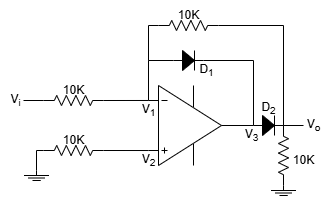
\includegraphics[width=1\linewidth]{Experiment_12/Circuit/Lab12a.drawio.png}
                \caption{Rectifier I}
                \label{cir:12a}
            \end{subfigure}
            \begin{subfigure}{0.4\textwidth}
                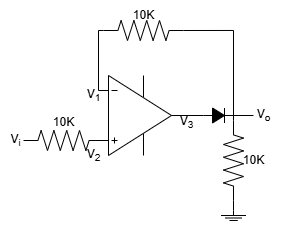
\includegraphics[width=1\linewidth]{Experiment_12/Circuit/Lab12b.drawio.png}
                \caption{Rectifier II}
                \label{cir:12b}
            \end{subfigure}
            \caption{Two different half-wave rectifier circuits}
        \end{figure}

    \subsubsection{Theoretical Analysis}
        \begin{enumerate}[a]
            \item \textbf{Inverting Amplifier}
        \end{enumerate}

\subsection{Experiment record}
    \subsubsection{Rectifier I}
    \begin{itemize}
        \item \textbf{Data Recorded}\newline
        In the circuit shown in figure \ref{cir:12a}, set the input signal frequency as 50Hz, and vary the amplitude, the output singal and the input signal is observed with the oscilloscope, and is shown in the following figure.\par
        \begin{figure}[H]
        \addtolength{\leftskip} {-3cm}
        \addtolength{\rightskip}{-3cm}
        \centering
            \begin{subfigure}{0.3\textwidth}
                \centering
                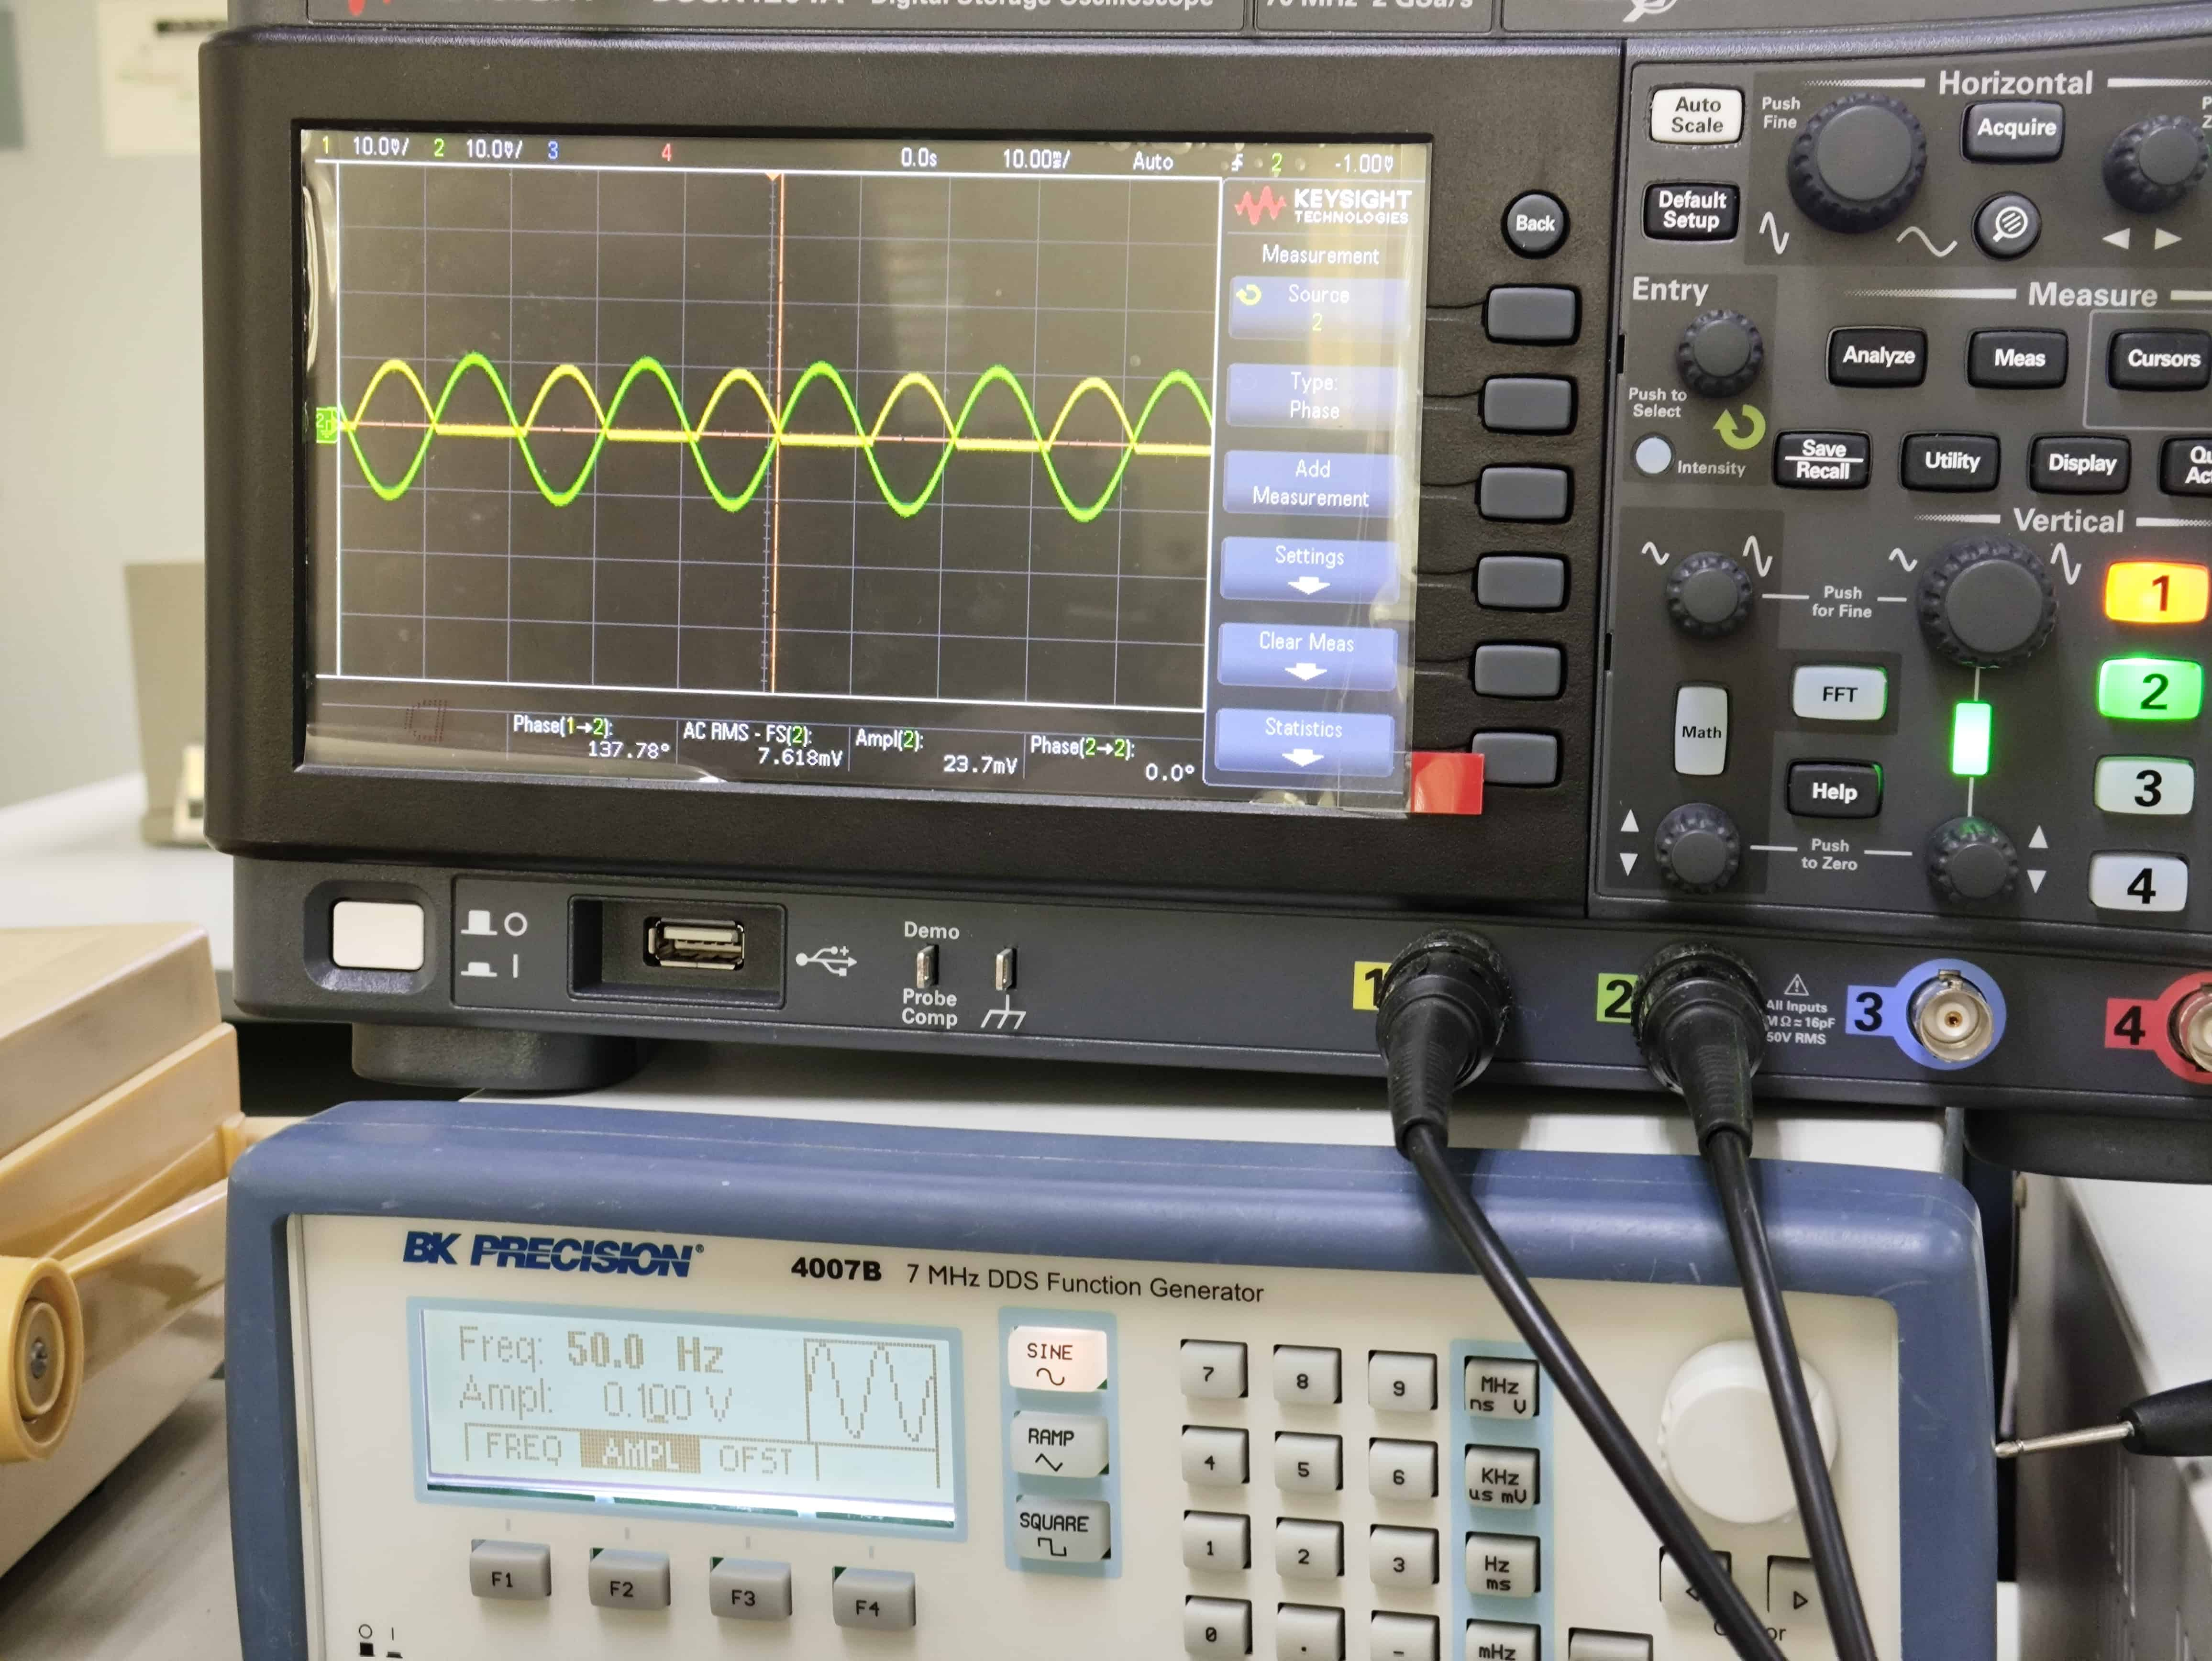
\includegraphics[width=1\linewidth]{Experiment_12/Images/RetA 50-0-min.jpg}
                \caption{Amplitude of 0.1V}
                \label{l120wf1}
            \end{subfigure}
            \begin{subfigure}{0.3\textwidth}
                \centering
                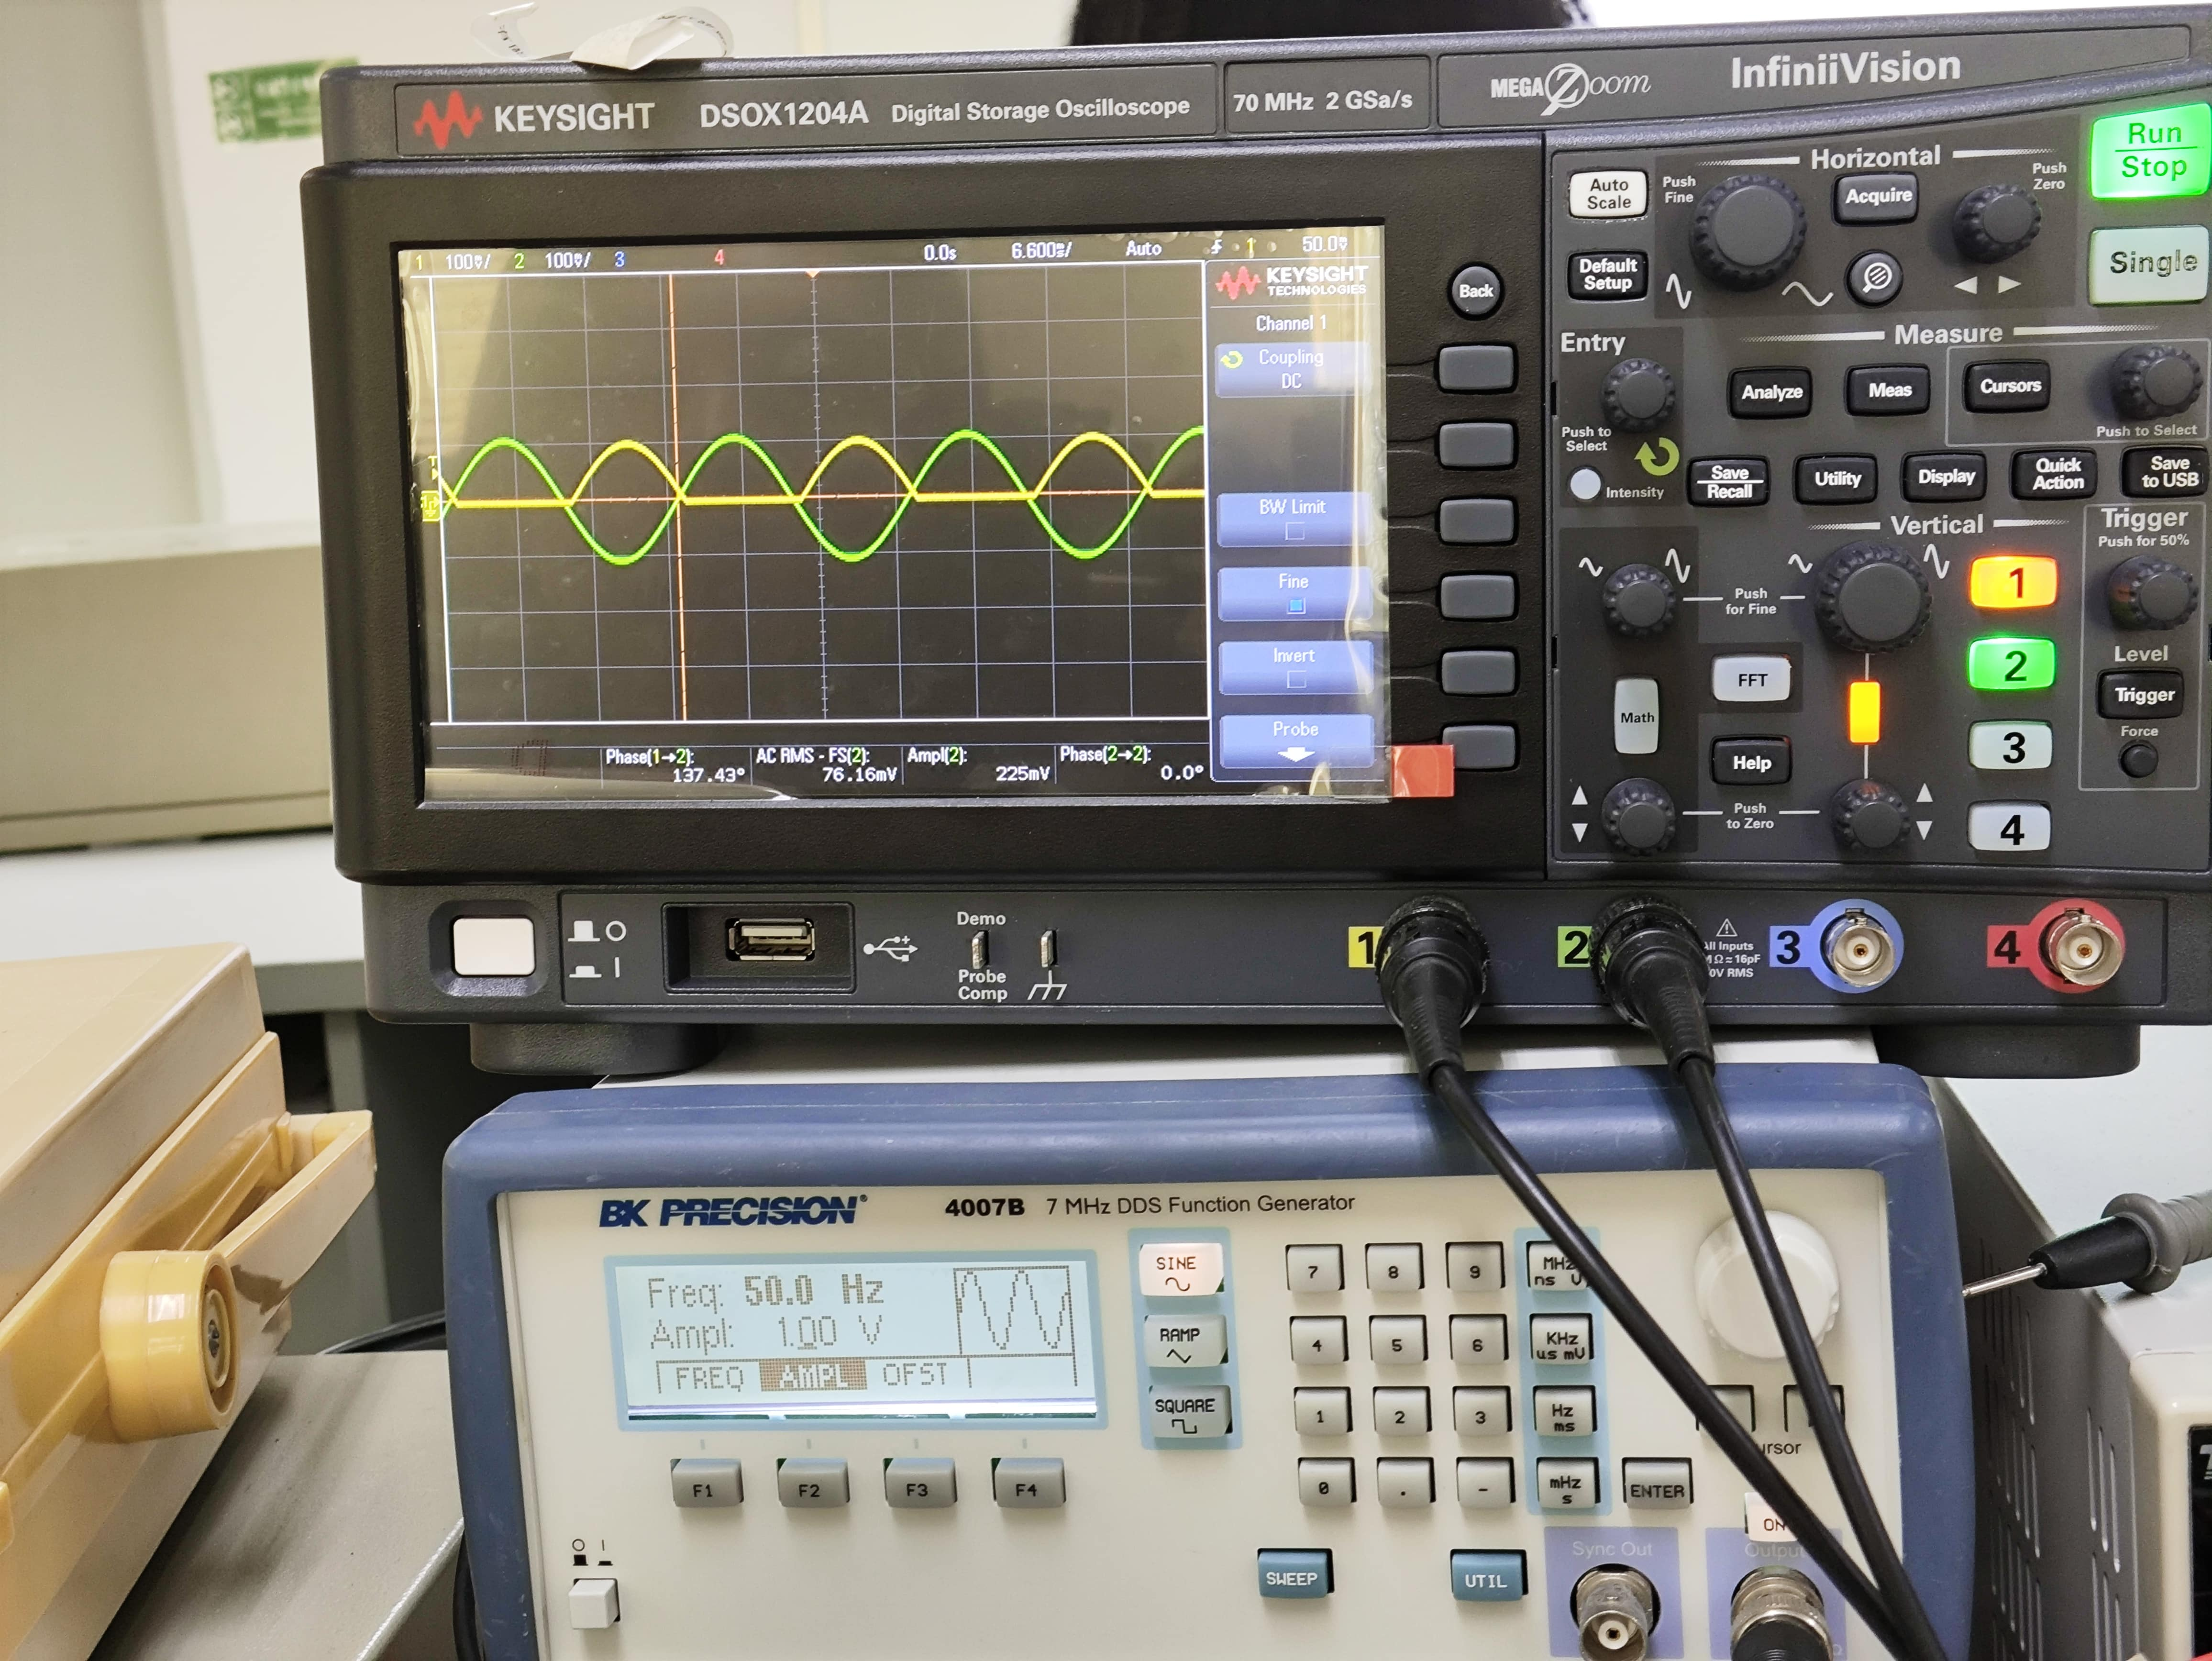
\includegraphics[width=1\linewidth]{Experiment_12/Images/RetA 50-1-min.jpg}
                \caption{Amplitude of 1V}
                \label{l121wf1}
            \end{subfigure}
            \begin{subfigure}{0.3\textwidth}
                \centering
                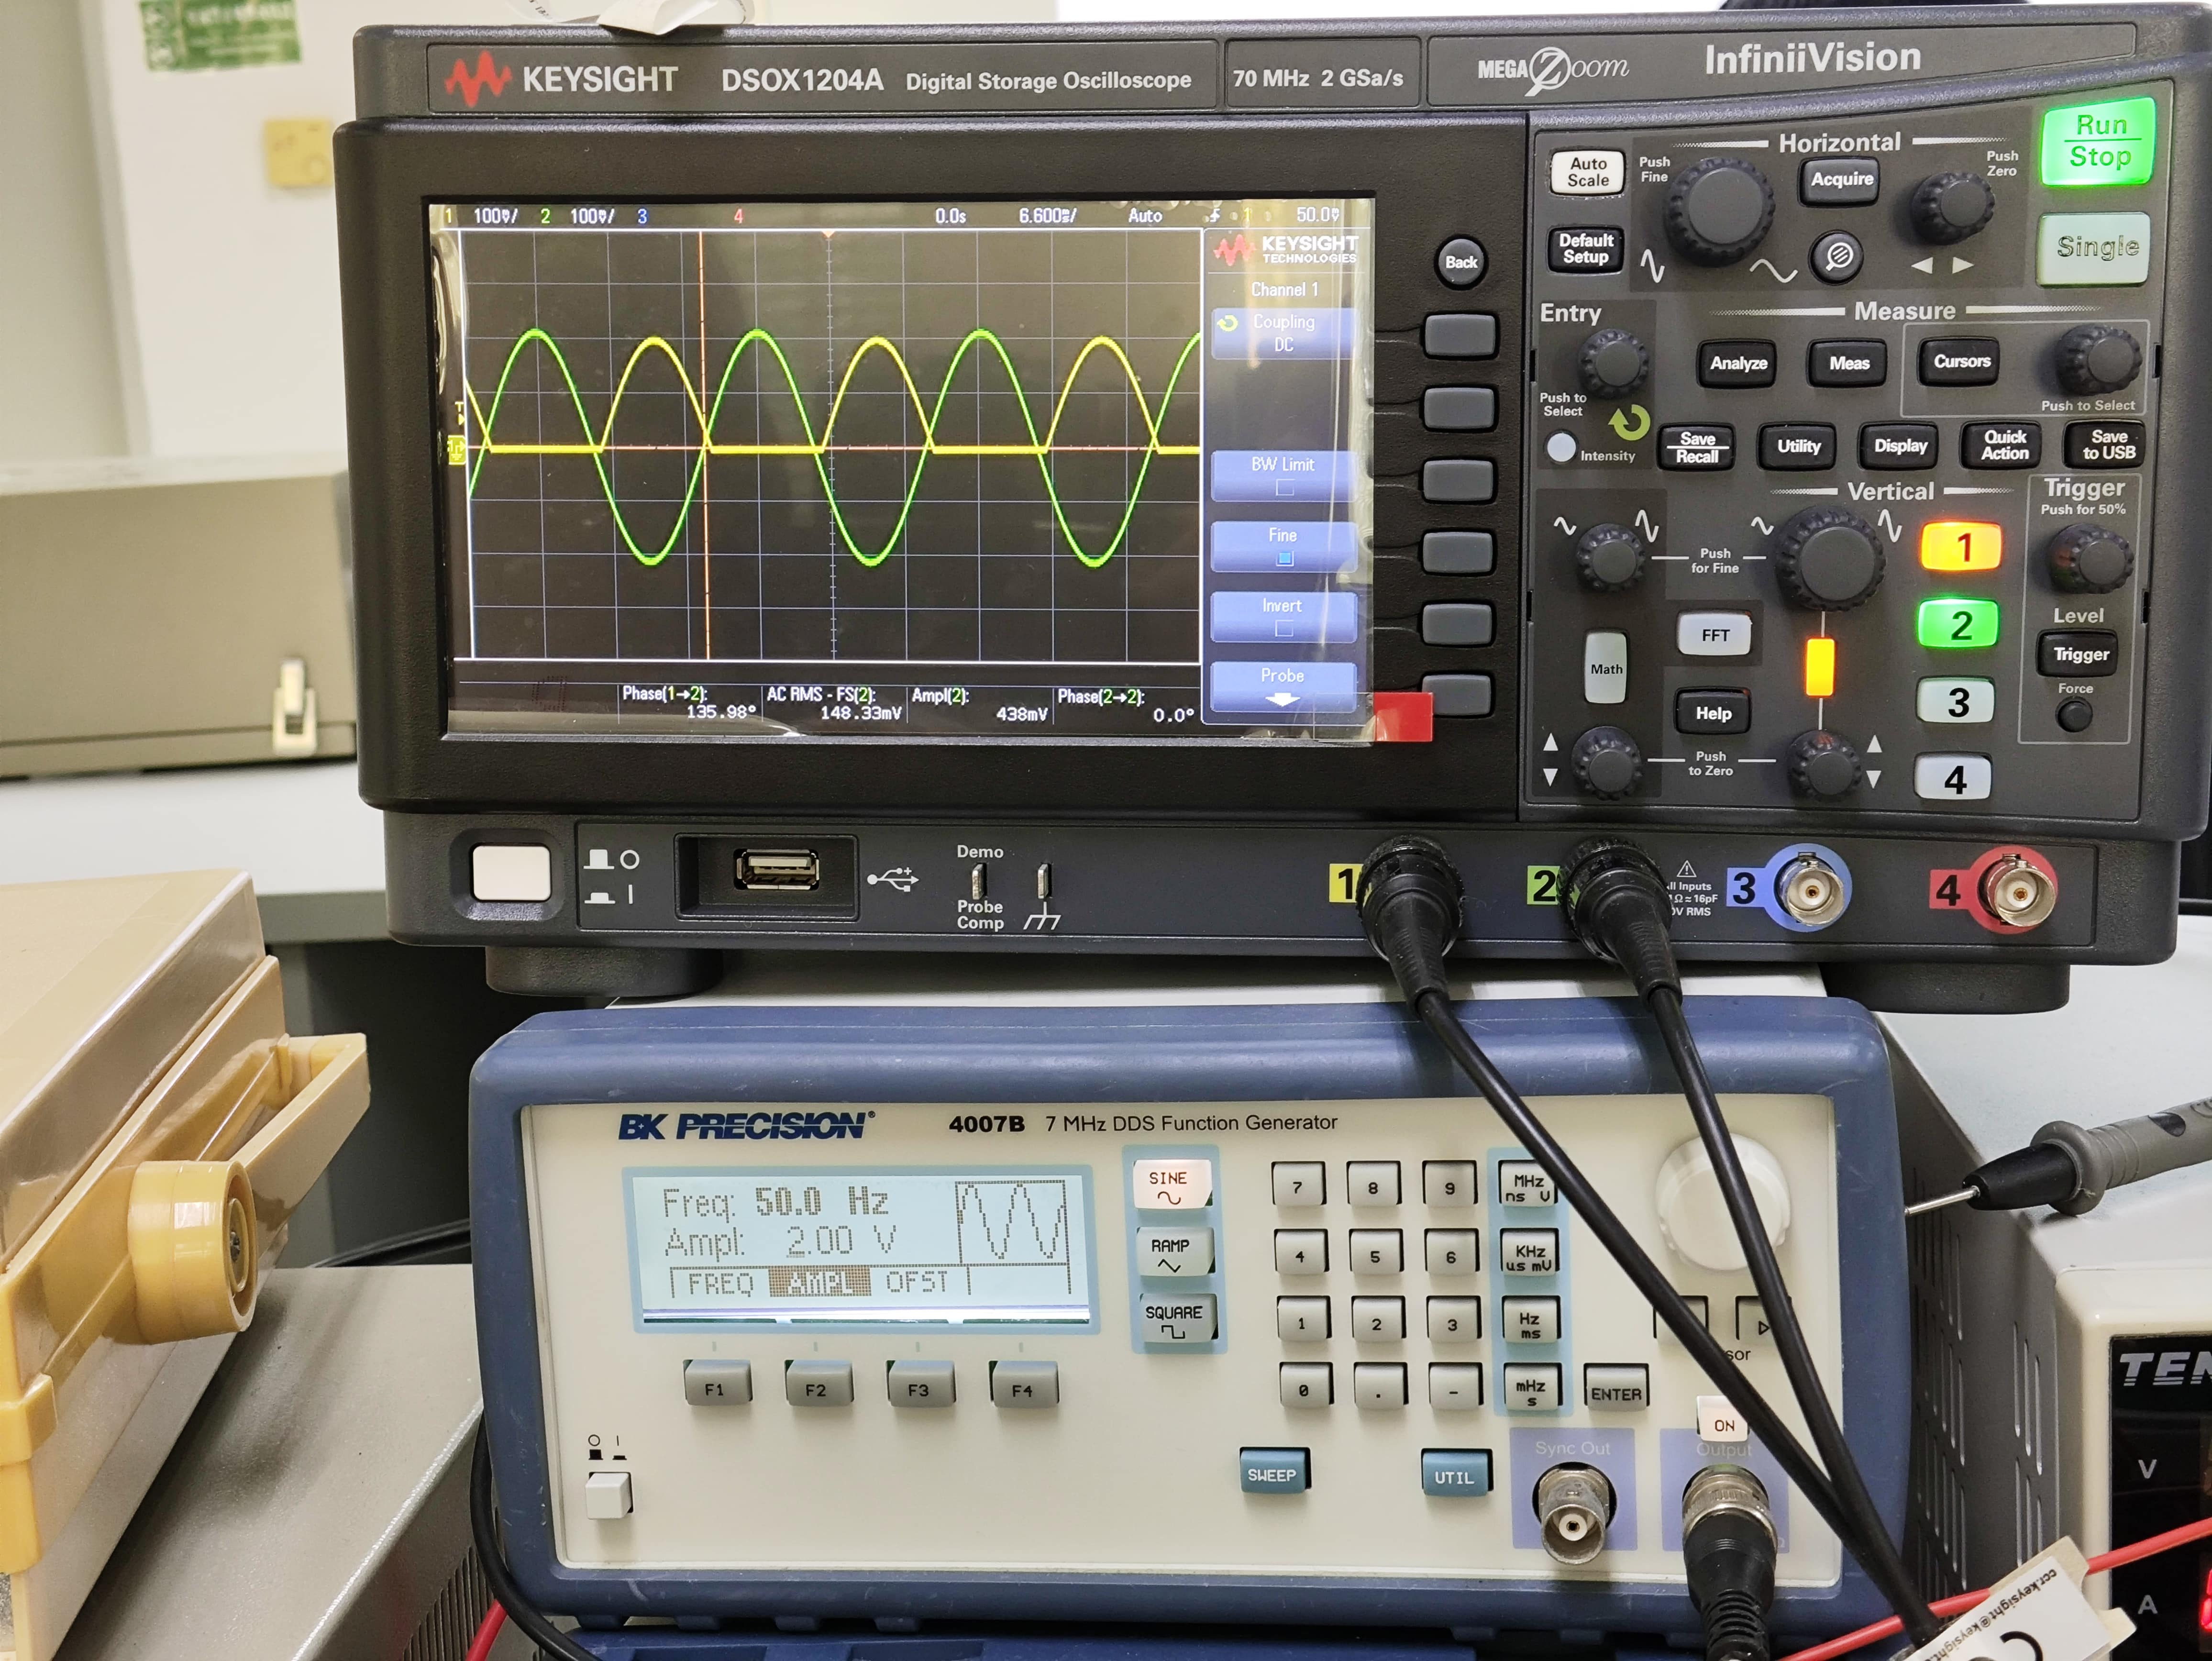
\includegraphics[width=1\linewidth]{Experiment_12/Images/RetA 50-2-min.jpg}
                \caption{Amplitude of 2V}
                \label{l122wf1}
            \end{subfigure}

            \begin{subfigure}{0.3\textwidth}
                \centering
                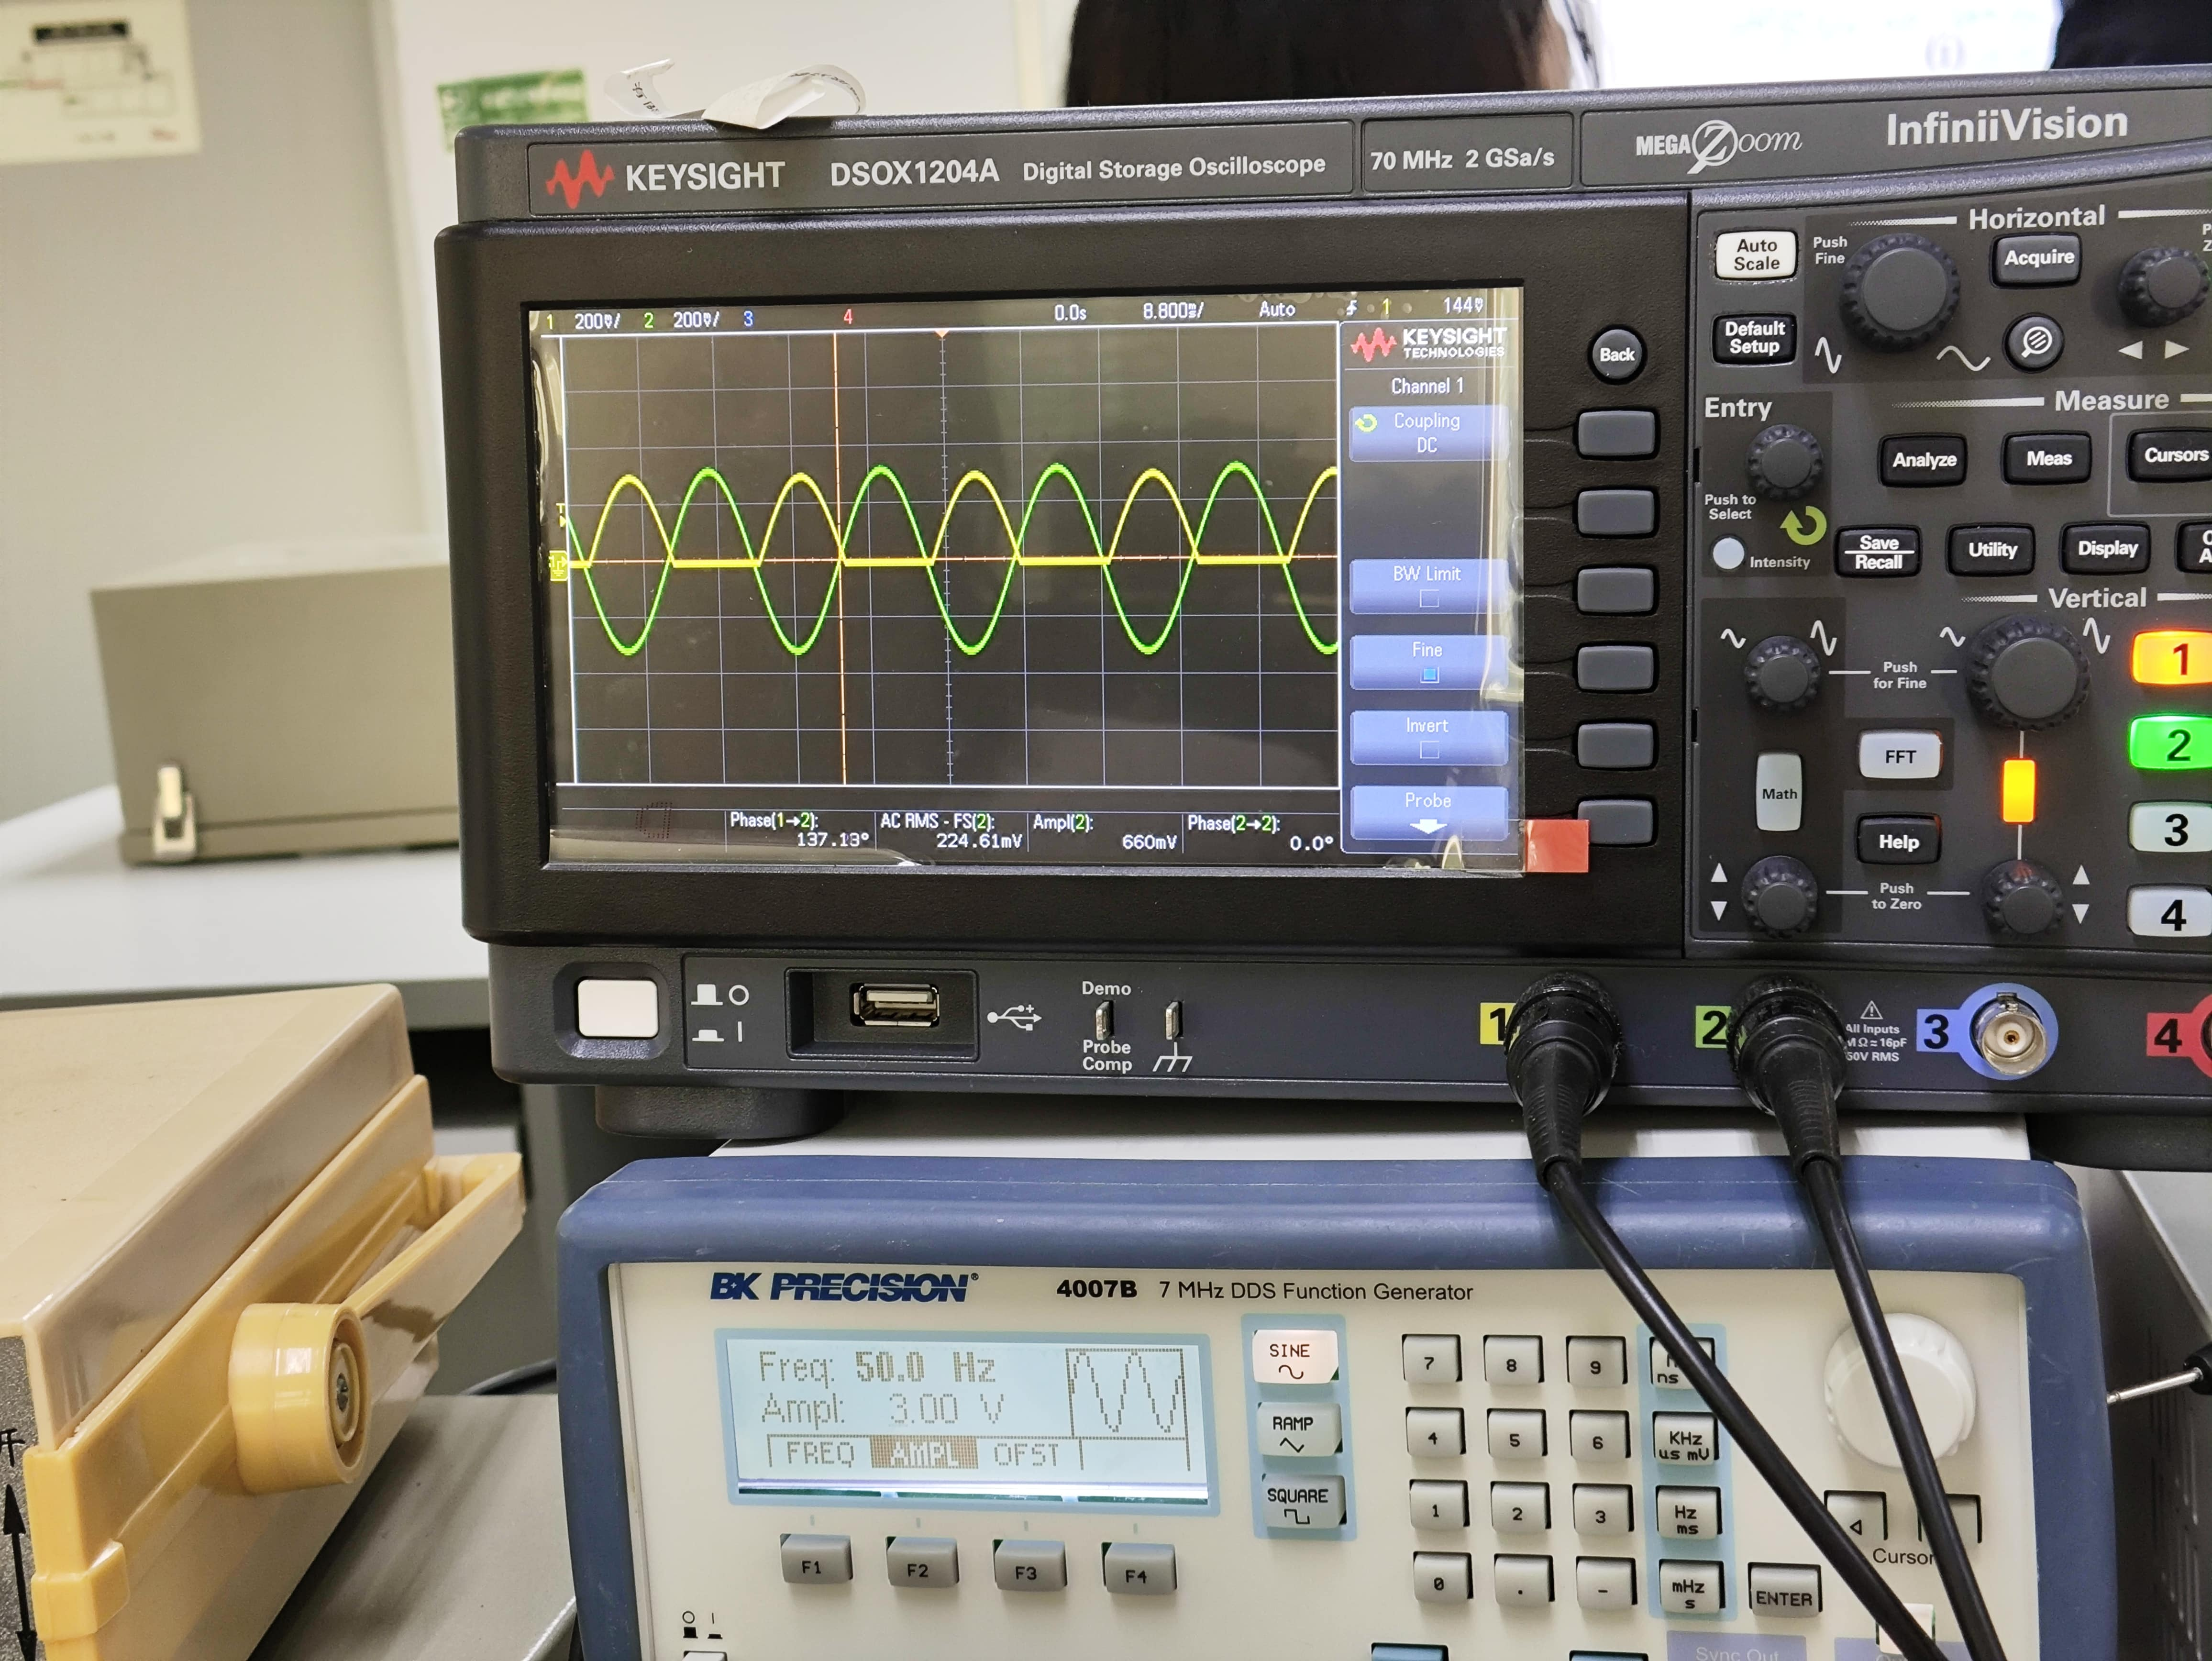
\includegraphics[width=1\linewidth]{Experiment_12/Images/RetA 50-3-min.jpg}
                \caption{Amplitude of 3V}
                \label{l123wf1}
            \end{subfigure}
            \begin{subfigure}{0.3\textwidth}
                \centering
                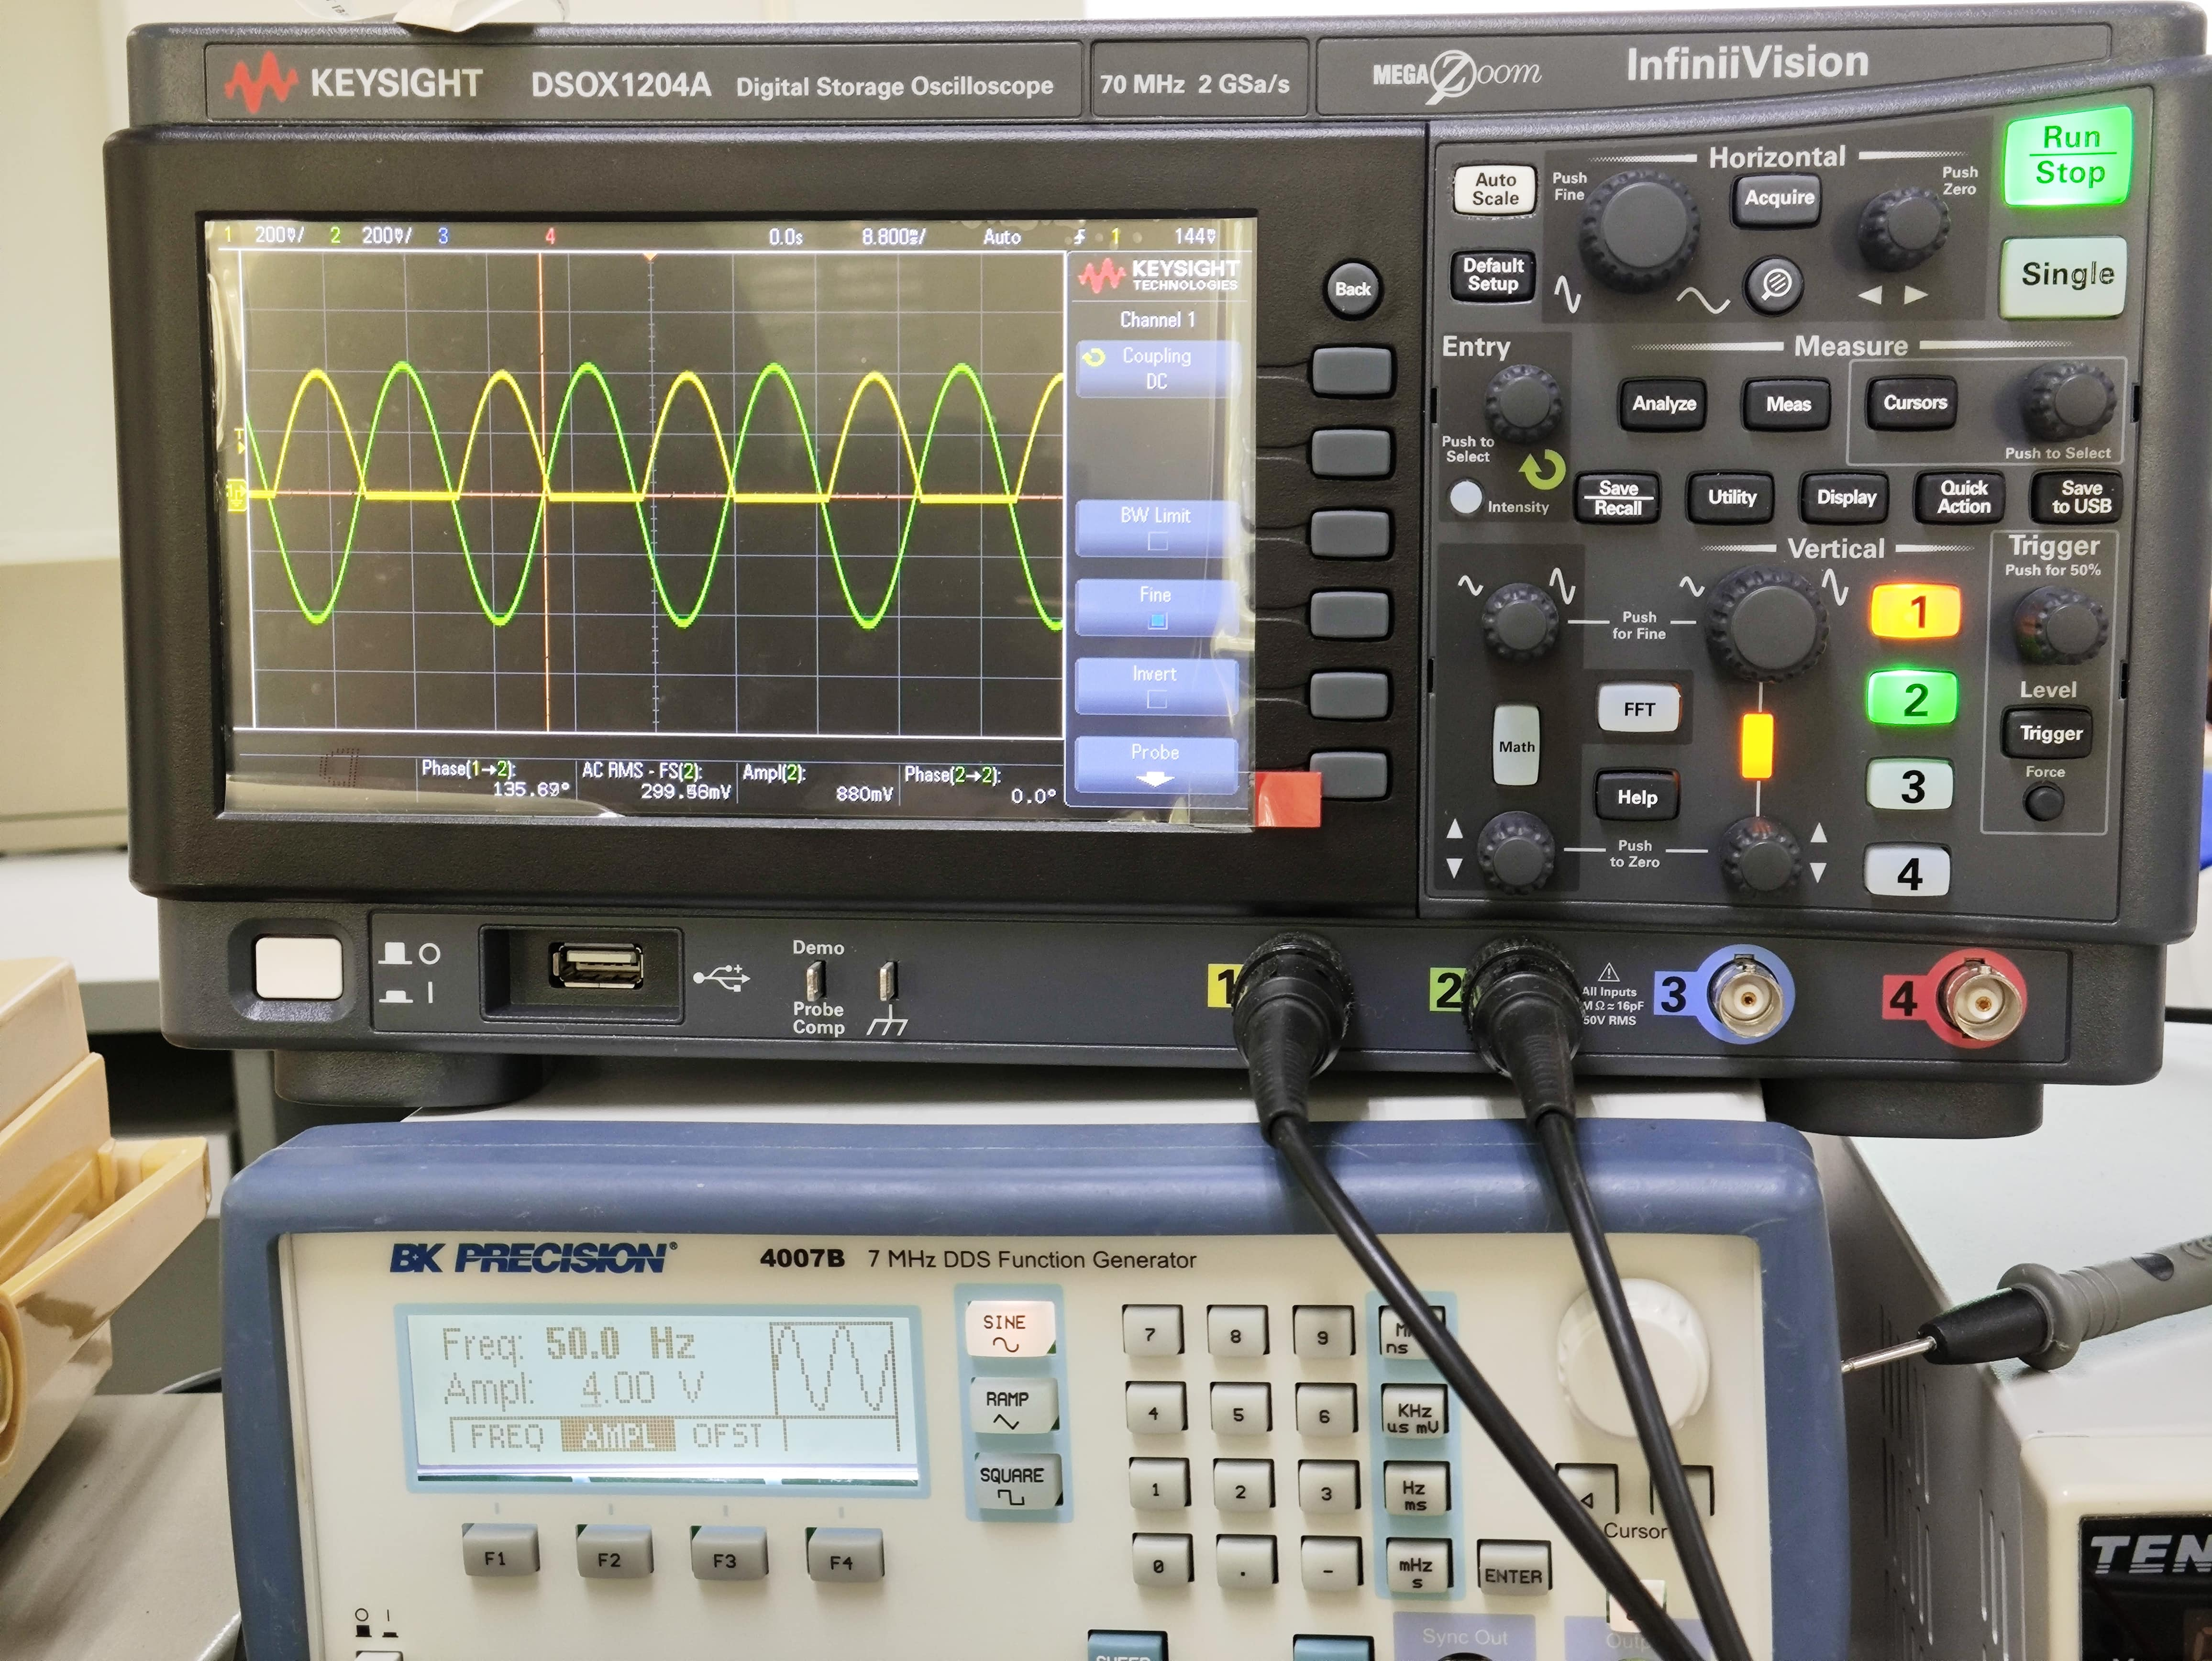
\includegraphics[width=1\linewidth]{Experiment_12/Images/RetA 50-4-min.jpg}
                \caption{Amplitude of 4V}
                \label{l124wf1}
            \end{subfigure}
            \begin{subfigure}{0.3\textwidth}
                \centering
                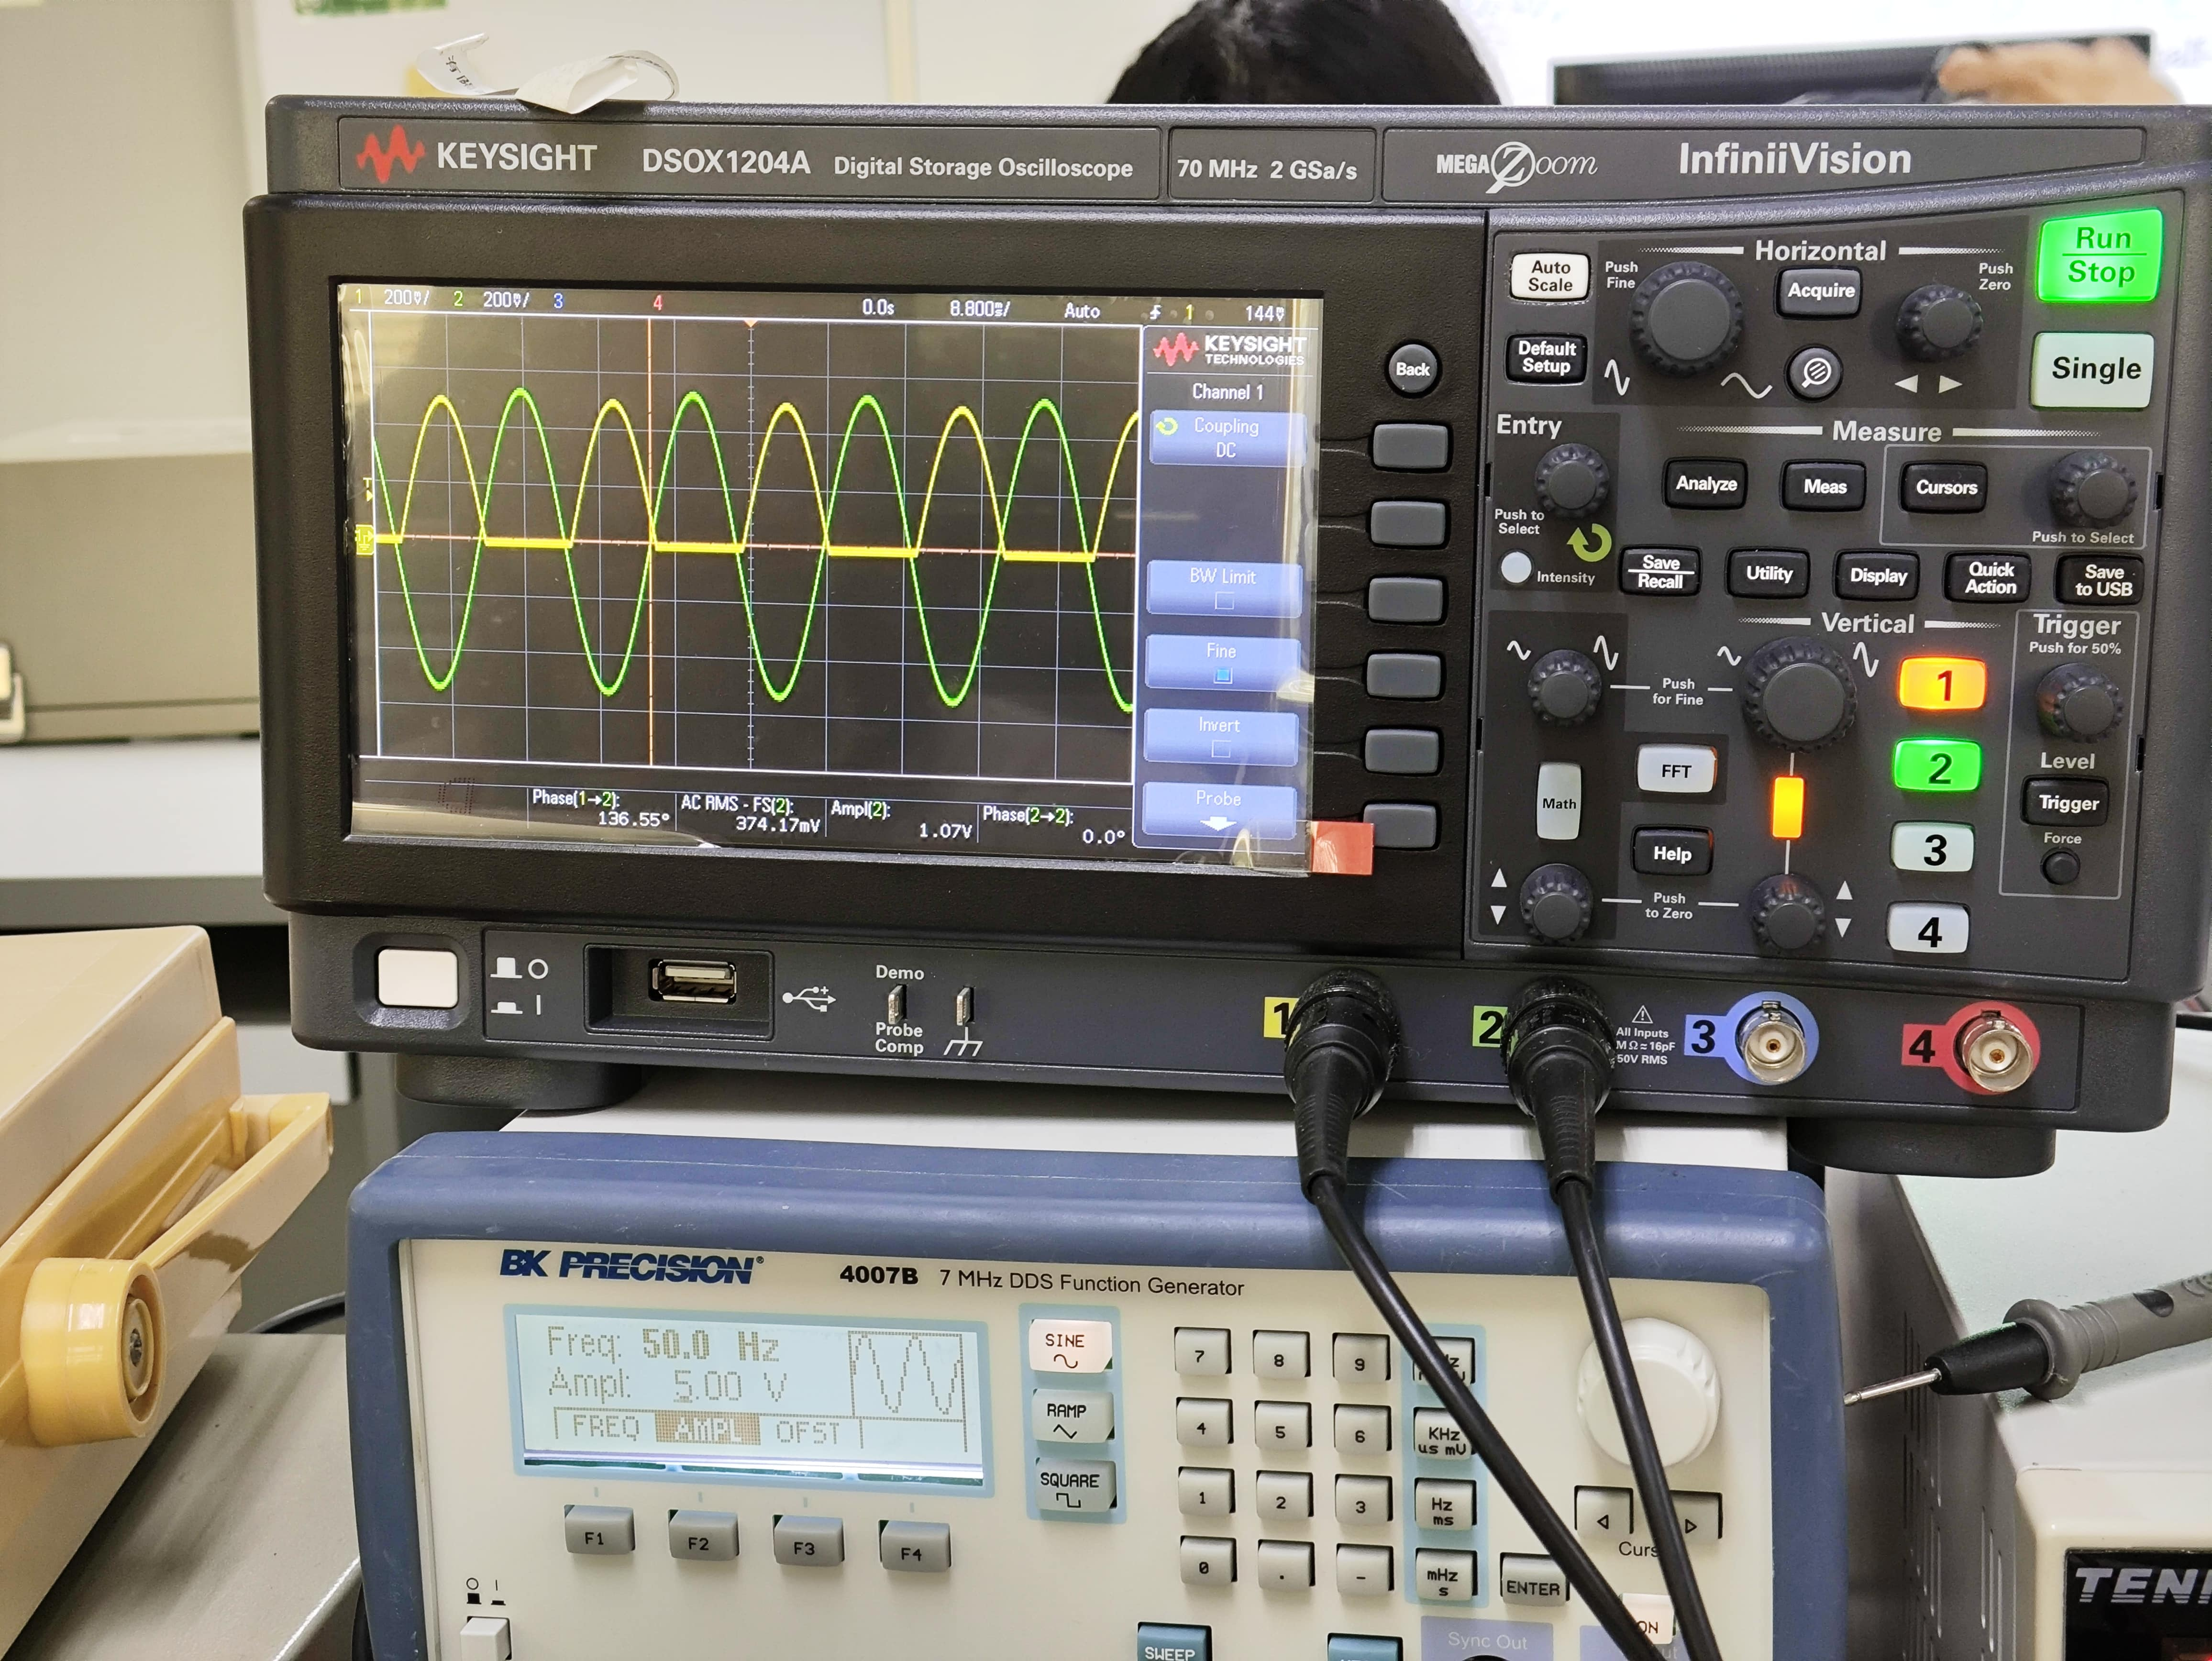
\includegraphics[width=1\linewidth]{Experiment_12/Images/RetA 50-5-min.jpg}
                \caption{Amplitude of 5V}
                \label{l125wf1}
            \end{subfigure}
        \end{figure}

        Then, we change the input signal into a DC voltage from -10V to 10V, and the voltage of important nodes are recorded in the following table.
        \begin{table}[H]
            \centering
            \begin{tabular}{l|rrrrrr}
                \midrule
                vi    & -10   & -5    & -1    & 1     & 5     & 10 \\
                \midrule
                v1    & -0.05 & 0     & -0.0015 & -0.003 & -0.05 & -0.05 \\
                v2    & 0     & 0     & 0     & 0     & 0     & 0 \\
                v3    & 10.5  & 5.583 & 1.518 & -0.5  & -0.58 & -0.62 \\
                vo    & 9.857 & 4.973 & 0.991 & -0.001 & -0.001 & -0.002 \\
                \bottomrule
                \end{tabular}%
            \caption{Recorded Data for the first rectifier}
            \label{tab:12a}
        \end{table}
        %\item \textbf{Data Analysis}\newline
    \end{itemize}

    \subsubsection{Rectifier II}
    \begin{itemize}
        \item \textbf{Data Recorded}\newline
        In the circuit shown in figure \ref{cir:12b}, set the input signal frequency as 50Hz, and vary the amplitude, the output singal and the input signal is observed with the oscilloscope, and is shown in the following figure.\par
        \begin{figure}[H]
        \addtolength{\leftskip} {-3cm}
        \addtolength{\rightskip}{-3cm}
        \centering
            \begin{subfigure}{0.3\textwidth}
                \centering
                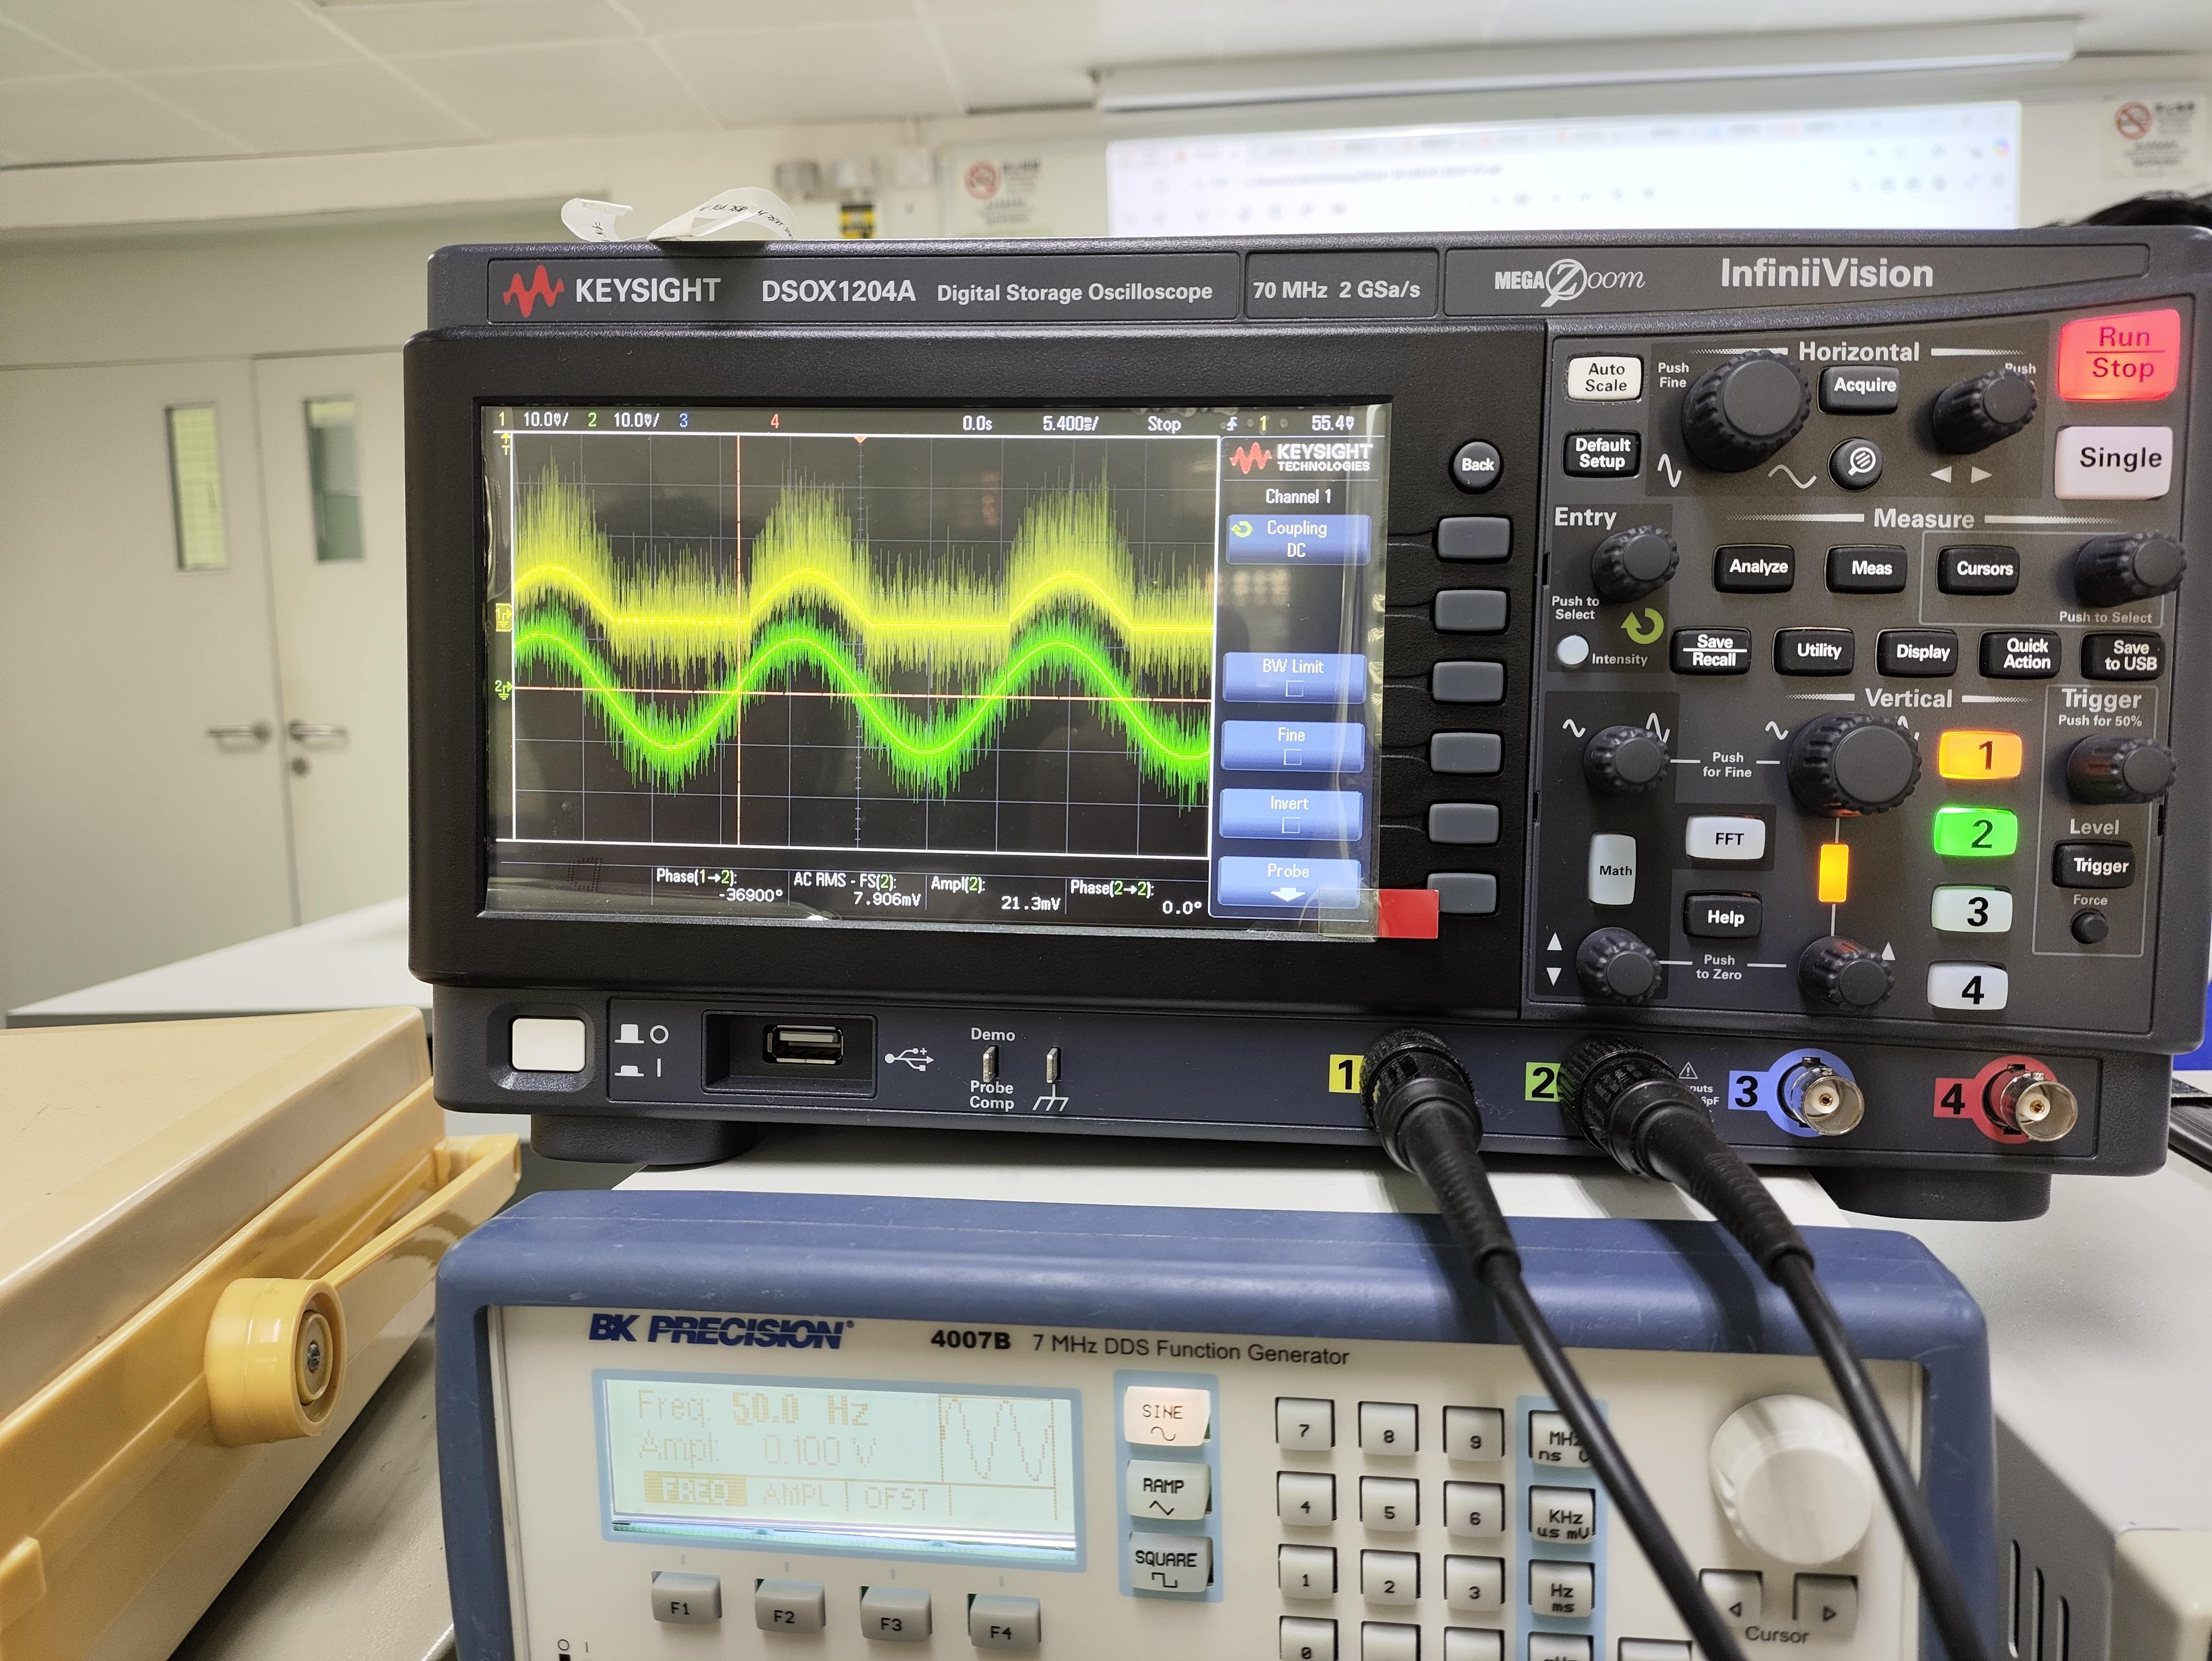
\includegraphics[width=1\linewidth]{Experiment_12/Images/RetB 50-0-min.jpg}
                \caption{Amplitude of 0.1V}
                \label{l120wf2}
            \end{subfigure}
            \begin{subfigure}{0.3\textwidth}
                \centering
                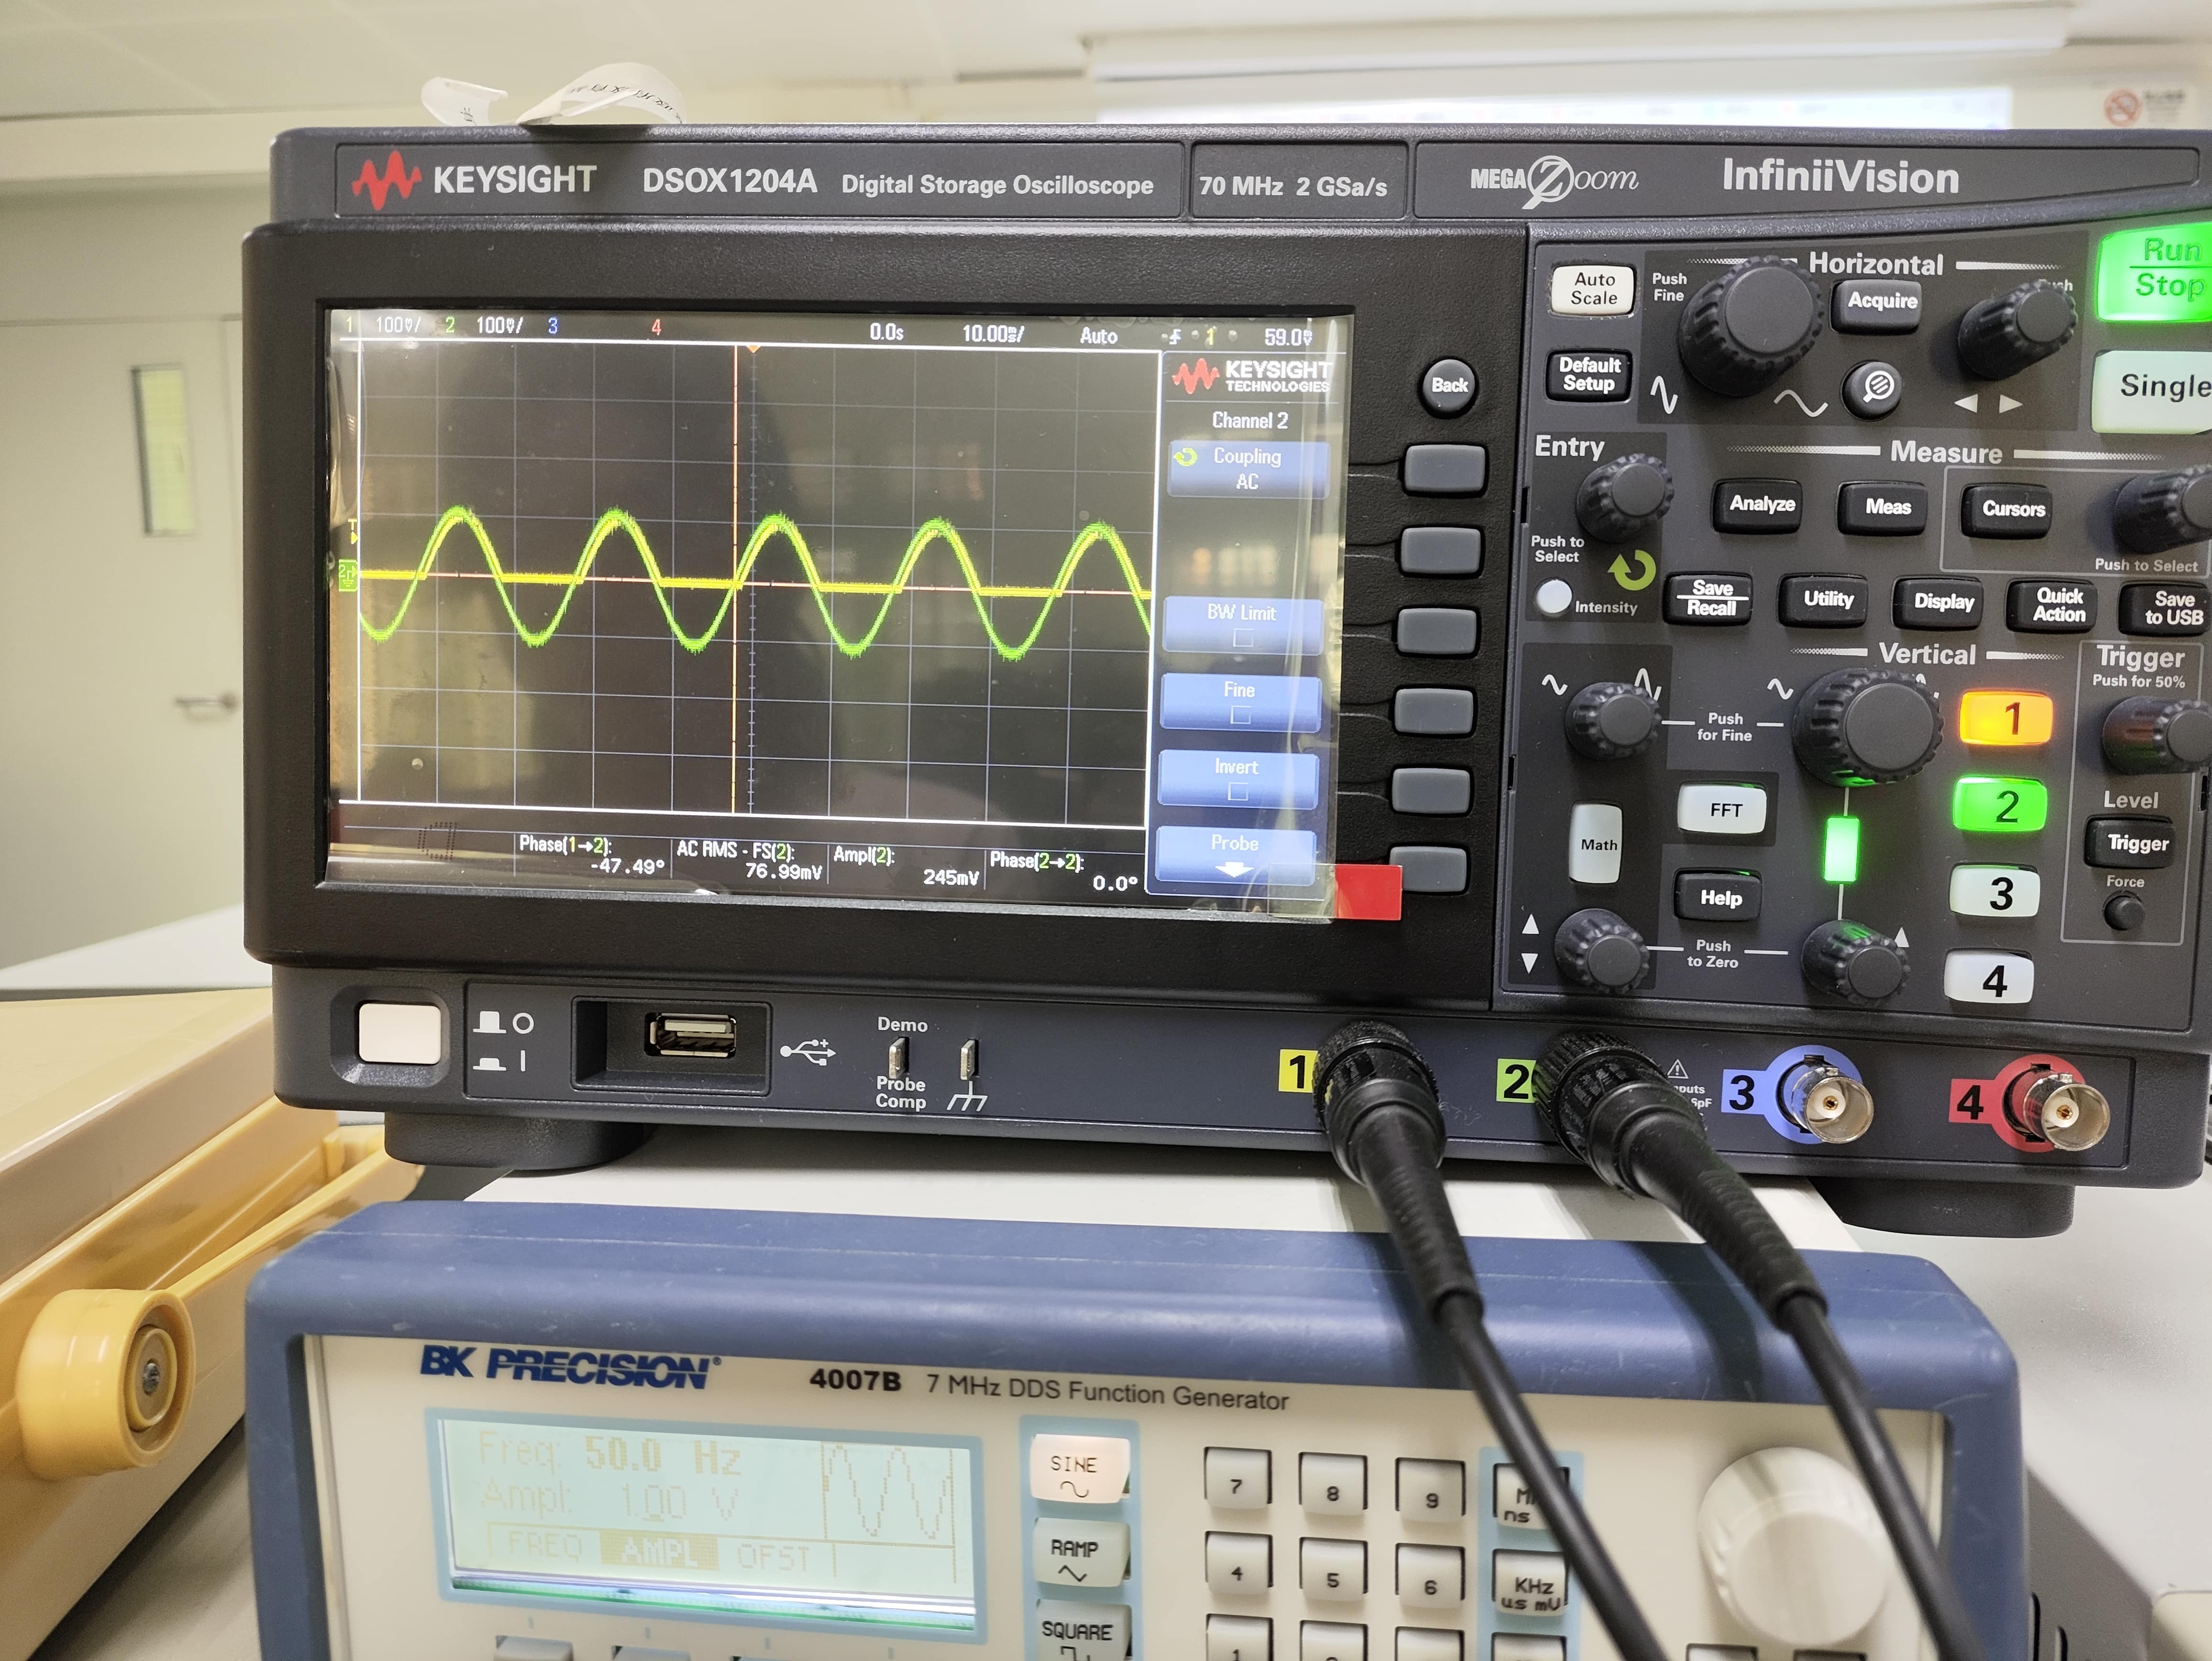
\includegraphics[width=1\linewidth]{Experiment_12/Images/RetB 50-1-min.jpg}
                \caption{Amplitude of 1V}
                \label{l121wf2}
            \end{subfigure}
            \begin{subfigure}{0.3\textwidth}
                \centering
                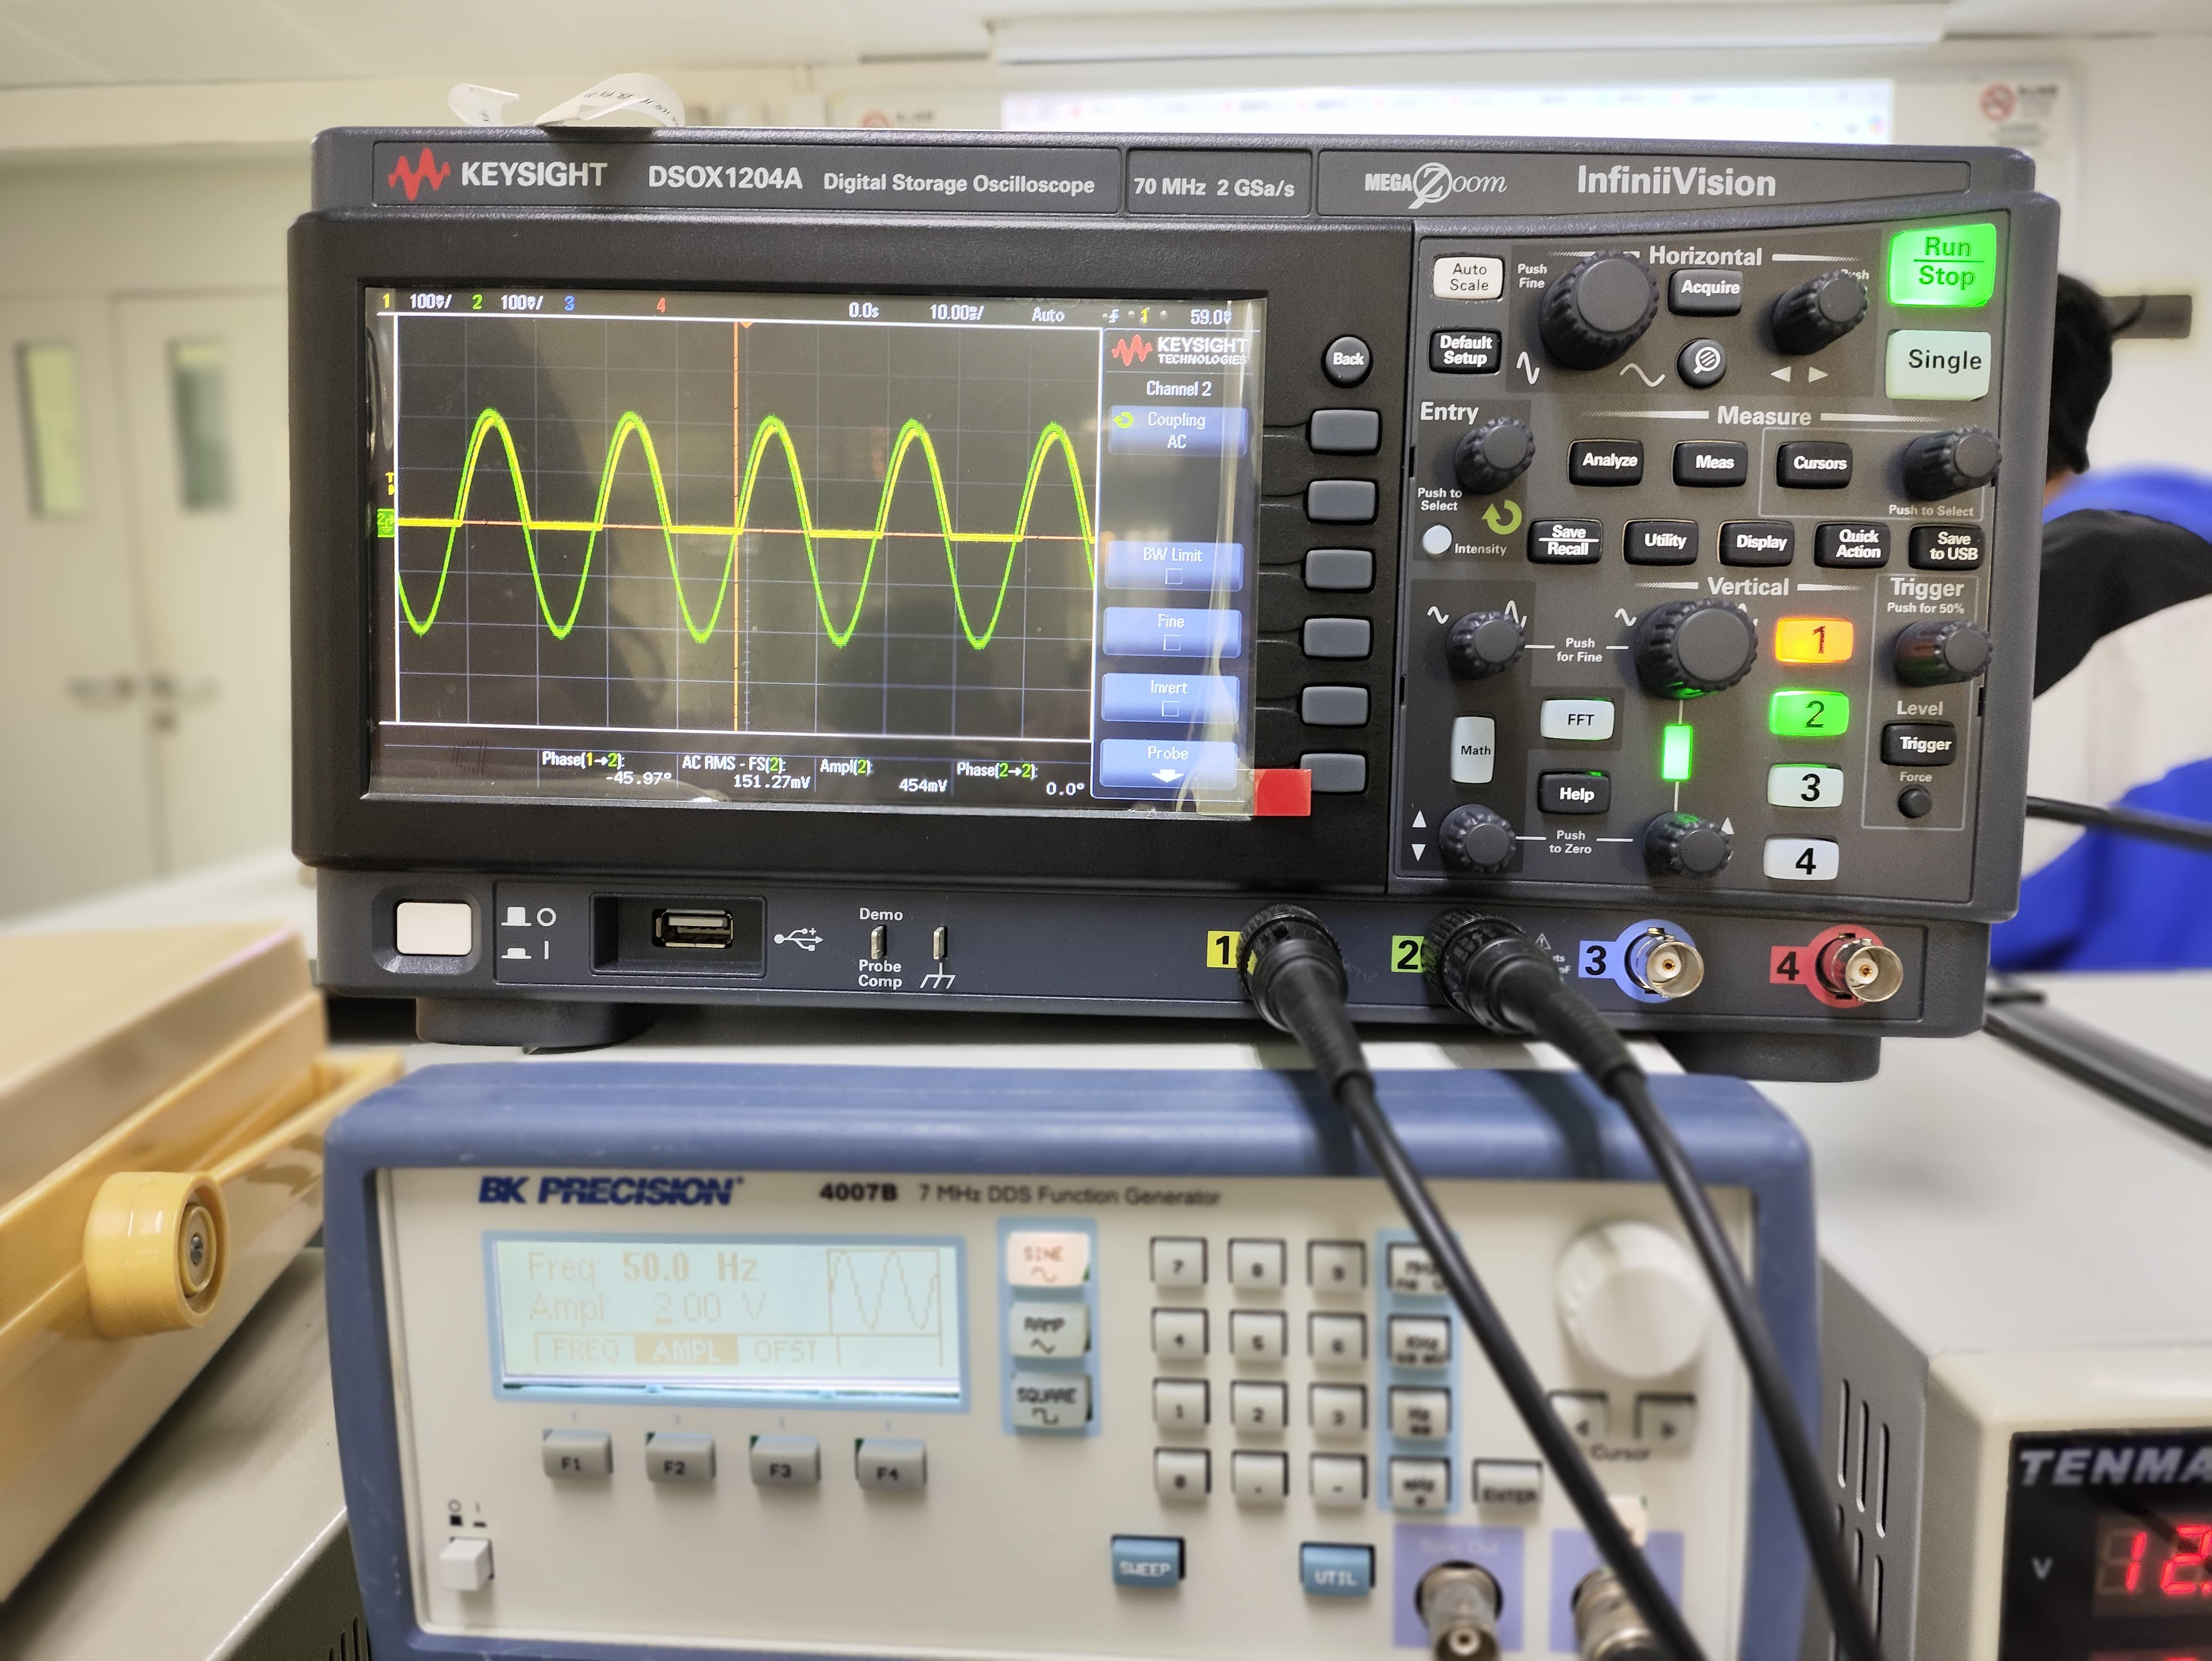
\includegraphics[width=1\linewidth]{Experiment_12/Images/RetB 50-2-min.jpg}
                \caption{Amplitude of 2V}
                \label{l122wf2}
            \end{subfigure}

            \begin{subfigure}{0.3\textwidth}
                \centering
                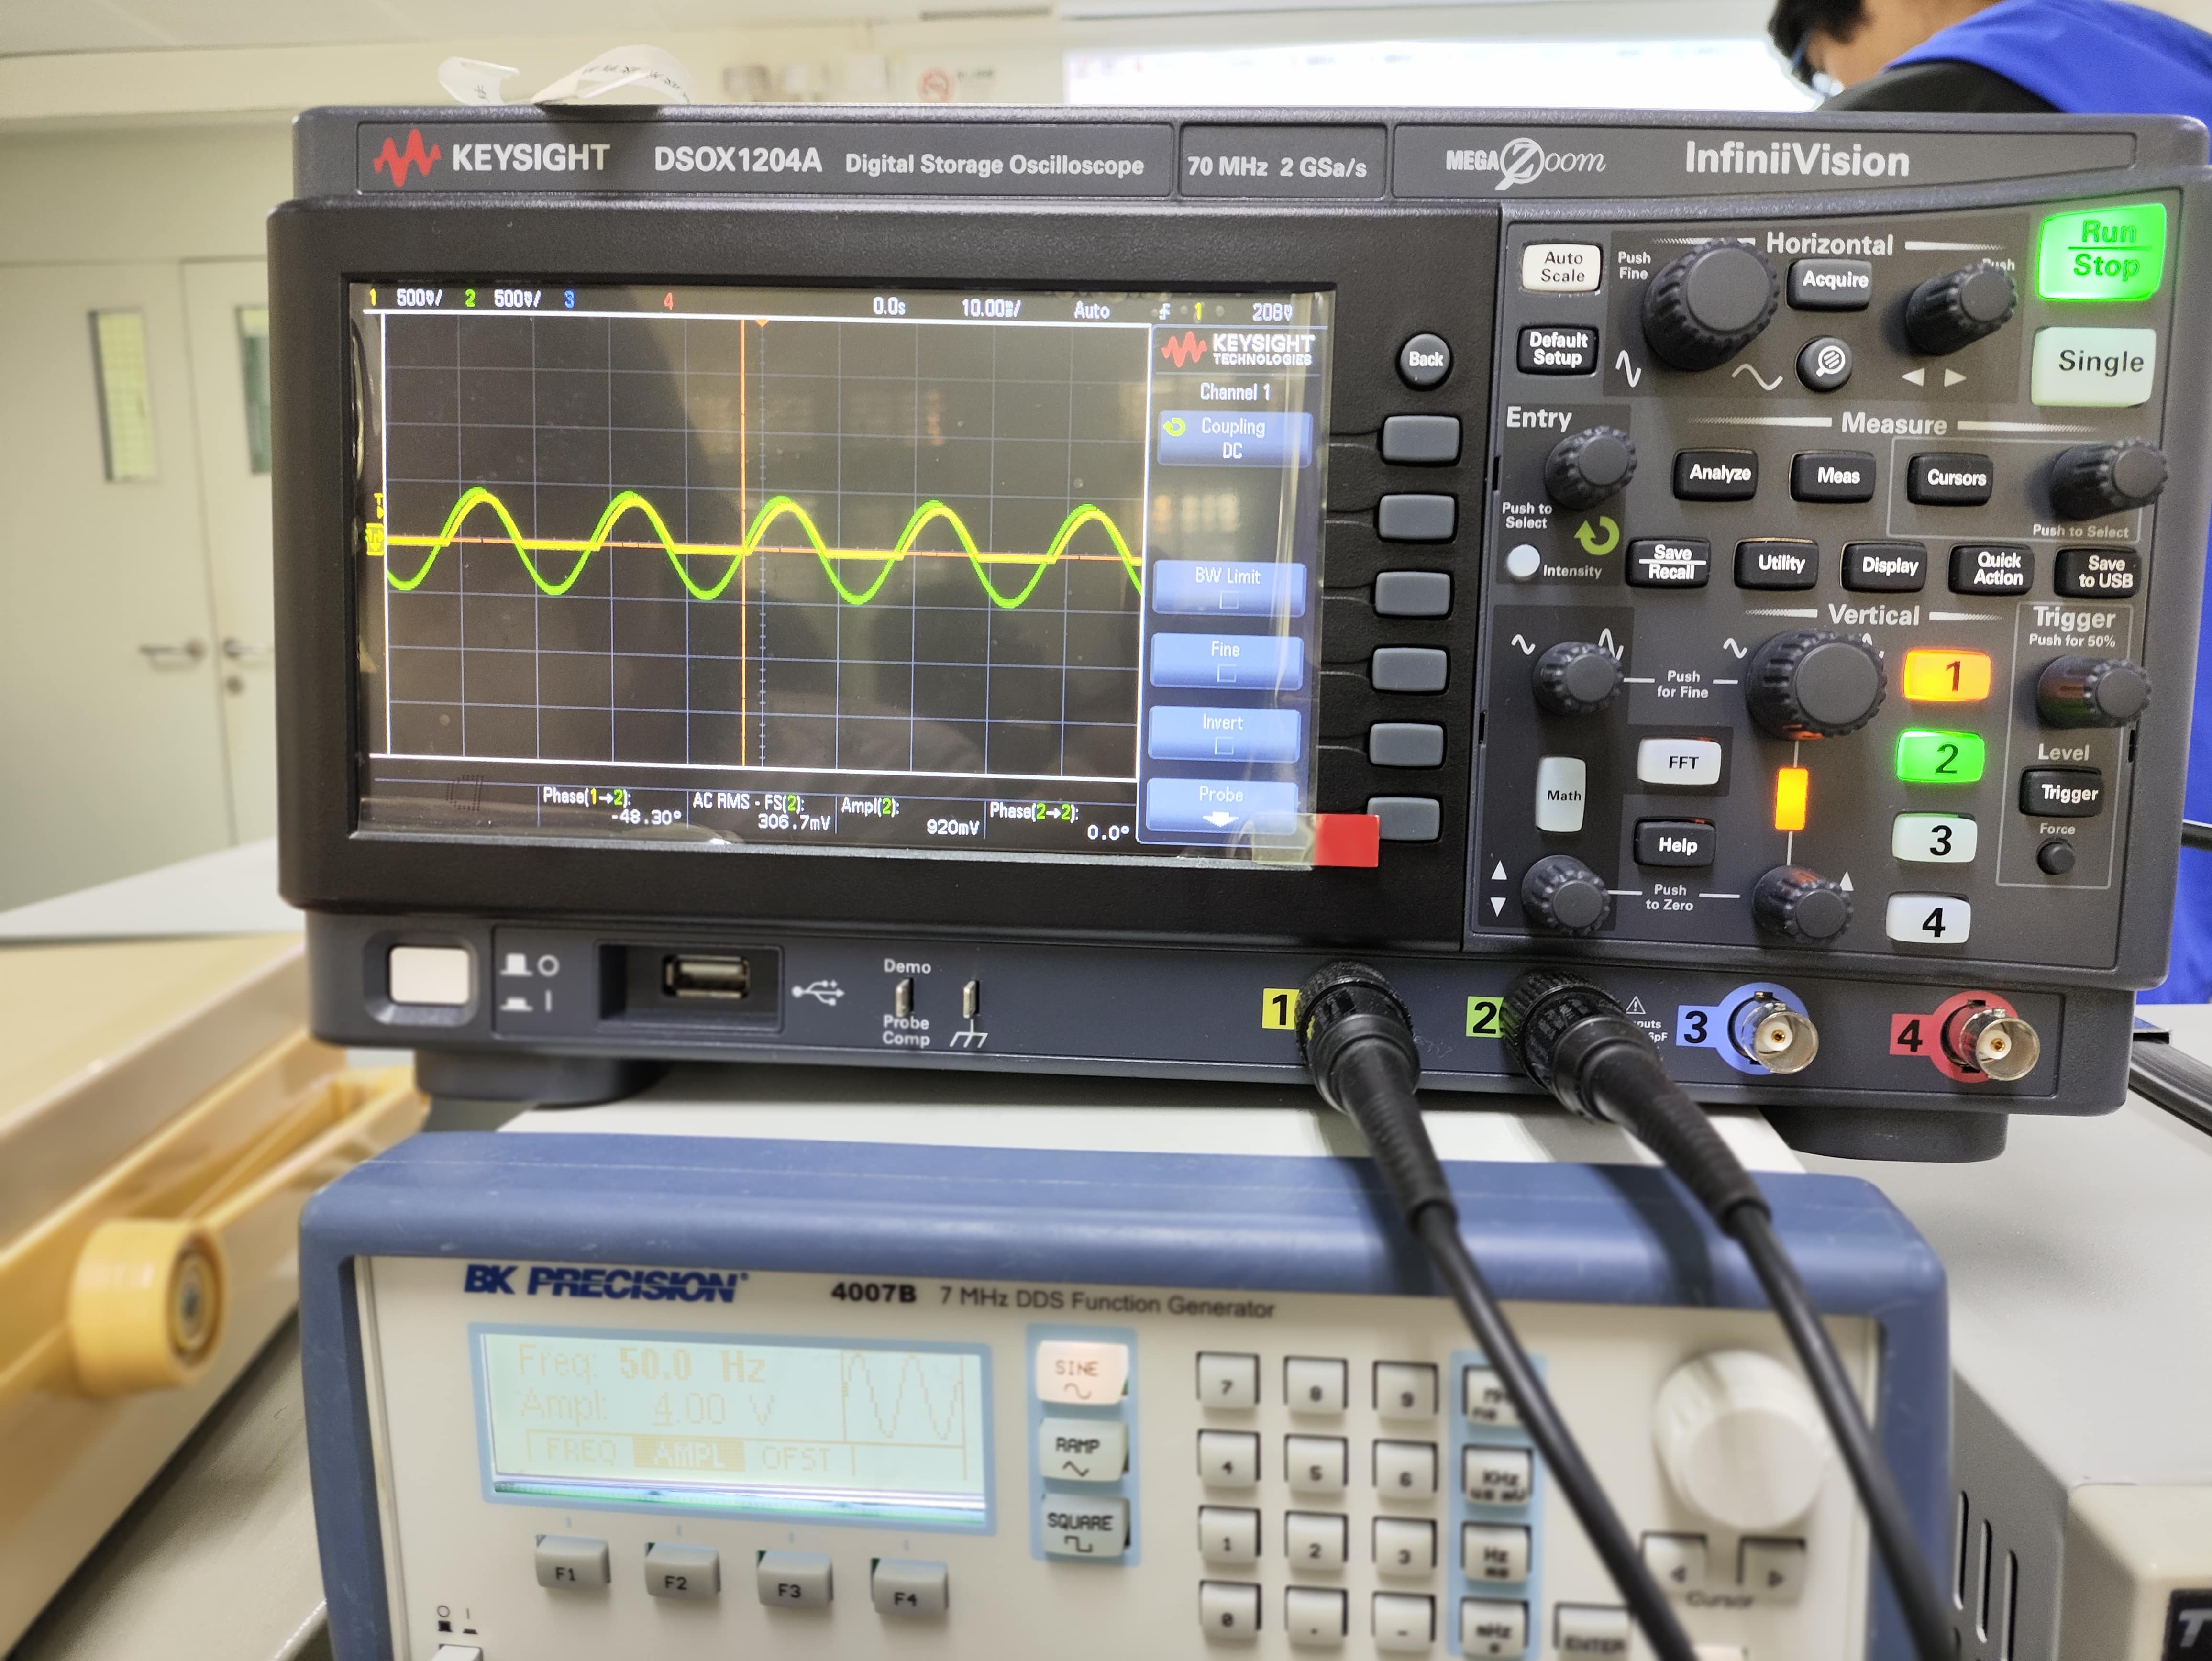
\includegraphics[width=1\linewidth]{Experiment_12/Images/RetB 50-4-min.jpg}
                \caption{Amplitude of 4V}
                \label{l124wf2}
            \end{subfigure}
            \begin{subfigure}{0.3\textwidth}
                \centering
                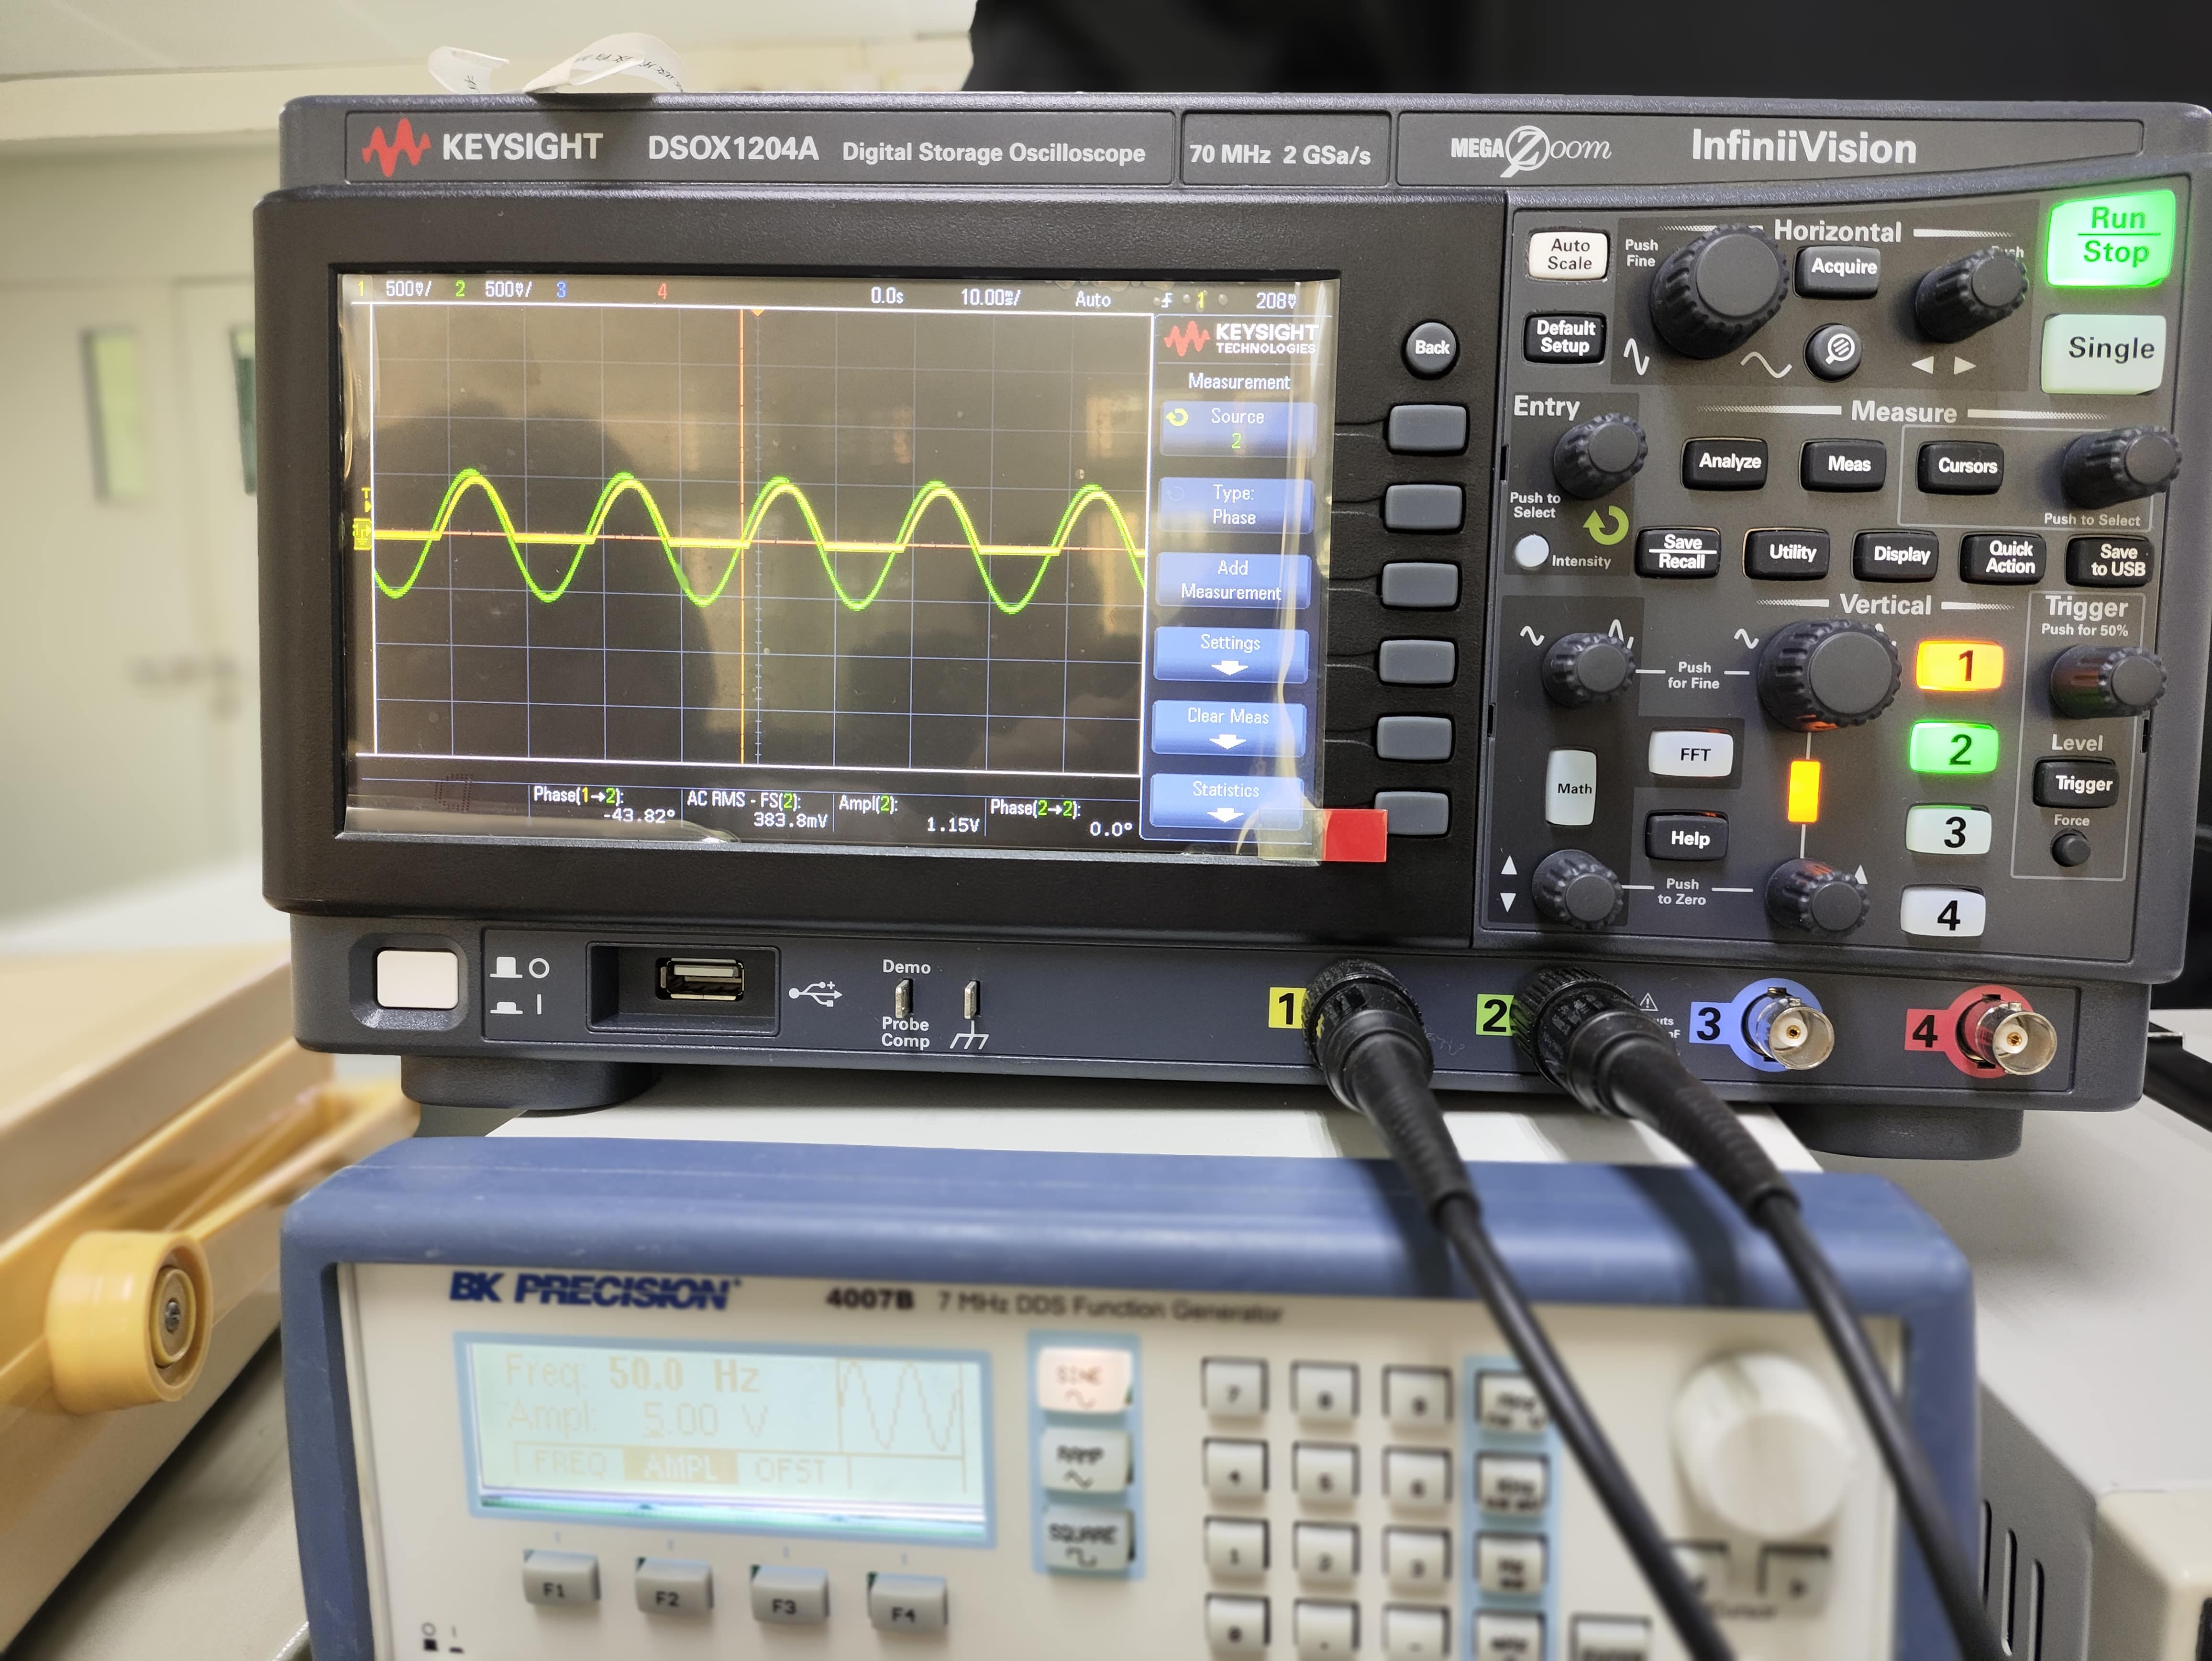
\includegraphics[width=1\linewidth]{Experiment_12/Images/RetB 50-5-min.jpg}
                \caption{Amplitude of 5V}
                \label{l125wf2}
            \end{subfigure}
        \end{figure}

        Then, we change the input signal into a DC voltage from -10V to 10V, and the voltage of important nodes are recorded in the following table.
        \begin{table}[H]
            \centering
            \begin{tabular}{l|cccccccc}
                \toprule
                vi & -12     & -10    & -5     & -1     & 1     & 5     & 10     & 12     \\
                \midrule
                v1 & -0.001  & 0      & 0      & 0      & 0.995 & 5     & 9.937  & 11.925 \\
                v2 & -11.969 & -9.99  & -4.996 & -0.995 & 0.996 & 4.99  & 9.995  & 10.582 \\
                v3 & -9.98   & -11.99 & -11.99 & -11.99 & 1.49  & 5.576 & 10.557 & 11.202 \\
                vo & 0       & 0      & 0      & 0      & 0.996 & 5     & 9.948  & 10.59  \\
                \bottomrule
            \end{tabular}
            \caption{Recorded Data for the second rectifier}
            \label{tab:12b}
        \end{table}
        %\item \textbf{Data Analysis}\newline
    \end{itemize}

\subsection{Experiment Conclusion}
    \subsubsection{Conclusion}
    In this experiment, we build the circuit for two precise rectifiers. And by obsering it's output signal respect to an small alternating input signal, we verify the precision of the rectifiers. The results are very closed to theoretical values.